%%%%%%%%%%%%%%%%%%%%%%%%%%%%%%%%%%%%%%%%%%%%%%%%%%%%%%%%%%%%%%%%%%%%%%%%%%%%%%%%%%%%%%%%%%%%%%%%%%%
% Chapter 2 -> Background
% Author: Eduardo G Gusmao
%%%%%%%%%%%%%%%%%%%%%%%%%%%%%%%%%%%%%%%%%%%%%%%%%%%%%%%%%%%%%%%%%%%%%%%%%%%%%%%%%%%%%%%%%%%%%%%%%%%
\chapter{Background}
\label{cha:background}

\graphicspath{{chapter2/figs/}}

% This chapter
In this chapter we provide background information required for the understanding of this thesis. First, we introduce the necessary biological concepts (Section~\ref{sec:gene.regulation}). Next, we present the biological experimental techniques which are the main sources of data used in our analyses (Section~\ref{sec:ngs.methods}). Then, we introduce the problem which we are going to address in this thesis -- the computational prediction of active transcription factor binding sites (TFBSs; Section~\ref{sec:computational.prediction.tfbs}). Subsequently, we discuss the state-of-the-art computational solutions to address this problem -- the computational footprinting methods (Section~\ref{sec:computational.footprinting.methods}). Finally, we close this chapter with concluding remarks on the definitions made in this chapter and a brief overview on our strategy to solve the problem of predicting active TFBSs (Section~\ref{sec:discussion.2}).

%%%%%%%%%%%%%%%%%%%%%%%%%%%%%%%%%%%%%%%%%%%%%%%%%%%%%%%%%%%%%%%%%%%%%
% Section: Gene Regulation
%%%%%%%%%%%%%%%%%%%%%%%%%%%%%%%%%%%%%%%%%%%%%%%%%%%%%%%%%%%%%%%%%%%%%
\section{Gene Regulation}
\label{sec:gene.regulation}

% Introduction & this section
In this thesis we focus on the biological field of gene regulation. Such research area focuses on the understanding of the cellular mechanisms behind the temporal and spatial expression of different genes on different cellular conditions. We start this section by describing the basic concepts of molecular biology (Section~\ref{sec:basic.concepts.molecular.biology}). Then, we describe the main biological processes regarding gene regulation (Section~\ref{sec:gene.regulation.transcription.factors}). Finally, we discuss the role of chromatin dynamics on such regulatory processes (Section~\ref{sec:chromatin}). The concepts presented in this section are based on~\cite{alberts2007} and~\cite{lodish2007}.

%%%%%%%%%%%%%%%%%%%%%%%%%%%%%%%%%%%%%%%%%%%%%%%%%%%%%%%%%%%%%%%%%%%%%
% Section: Basic Concepts of Molecular Biology
%%%%%%%%%%%%%%%%%%%%%%%%%%%%%%%%%%%%%%%%%%%%%%%%%%%%%%%%%%%%%%%%%%%%%
\subsection{Basic Concepts of Molecular Biology}
\label{sec:basic.concepts.molecular.biology}

% Introduction
In this thesis we focus on two important macromolecules which are found inside cells: proteins (composed of amino acids) and nucleic acids (composed of nucleotides). Proteins assume many roles: catalysis of chemical reactions (enzymes), metabolite processing, cell signaling, regulation of the production of more proteins, structural function and others. Given such great variety of roles, one might regard these macromolecules as fundamental for the maintenance of living organisms. There are two types of nucleic acids: the deoxyribonucleic acid (DNA) and ribonucleic acid (RNA). The main function of the DNA is to store the hereditary information of the organism. It is based on such information that new proteins are generated. The RNA have many important functions; however we will not focus on this molecule in this work.

% DNA structure
The DNA molecule is formed by a double helix of paired nucleotide chains, each of which composed of the nucleotide types: adenine (A), cytosine (C), guanine (G) and thymine (T). Each nucleotide is composed of a sugar (deoxyribose), a phosphate group and a nitrogenous base (which determines the nucleotide type). Within each DNA strand of the double helix, nucleotides are connected through phosphodiester bonds (strong covalent bonds). Between each DNA strand, nucleotides are paired and connected through hydrogen bonds (weaker than covalent bonds). Cytosines always pair with guanines and adenines always pair with thymines. Because nucleotides are paired between the double helix structure, it is common to refer to nucleotides as base pairs (bp). Figure~\ref{fig:alberts_dna_structure} depicts a graphical representation of the DNA molecule.

% Figure - DNA structure
\begin{figure}[h!]
\centering
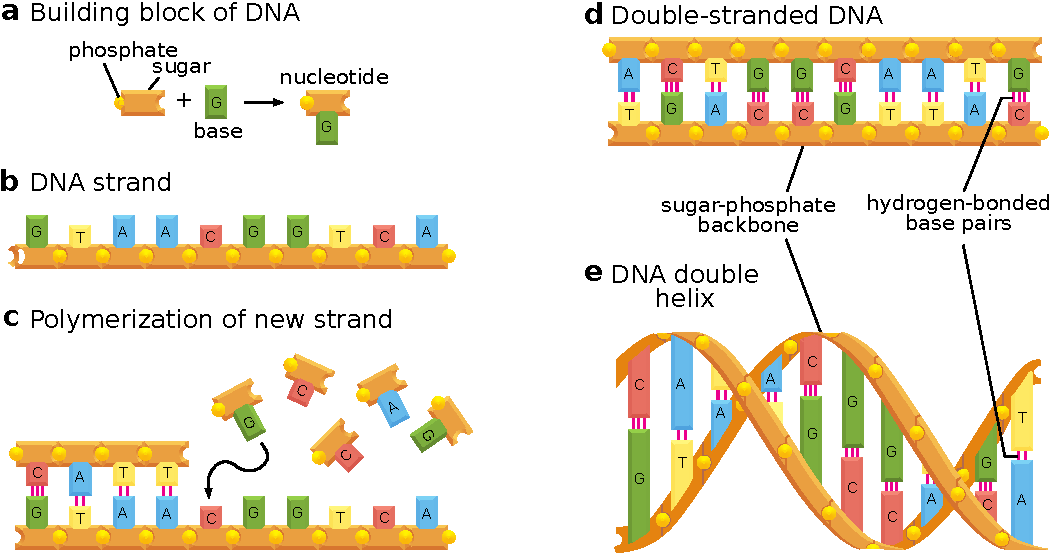
\includegraphics[width=0.99\textwidth]{alberts_37_dna_structure}
\caption[DNA structure]{\textbf{DNA structure.} (\textbf{a}) Representation of the DNA's building block -- the nucleotide. (\textbf{b}) Multiple nucleotides from all possible types (A, C, G and T) form a single strand of DNA, which in humans are as long as \approxy$250,000,000$ nucleotides. (\textbf{c}) The DNA generally occurs as a double strand. The biological process of polymerization allows the addition of nucleotides to a single strand, forming the DNA double strand. Cytosines (C) always pair with guanines (G) connected through three hydrogen bonds (pink lines); and adenines (A) always pair with thymines (T) through two hydrogen bonds. (\textbf{d}) Linear scheme of the double DNA strands. (\textbf{e}) Double helix structure of the double-stranded DNA molecule. This is the general structure in which the DNA occurs in nature. \emph{Source:~\cite{alberts2007}} (modified to fit thesis format and/or clarify key points).}
\label{fig:alberts_dna_structure}
\end{figure}

% Protein structure dictates function
Proteins are chemical compounds with high molecular weight formed by a variable-length chain of amino acids. The amino acids that forms the proteins are composed of a central carbon atom which binds to a hydrogen, a carboxyl group, an amine group and a side chain. The side chain may be of various types and dictates the type of the amino acid. There are $20$ amino acid types commonly found at proteins. The specific order of each amino acid type in a protein determines its three-dimensional structure. It is well-known that the protein's function is directly related to its structure. The simple substitution of one amino acid in the proteic chain is sufficient to modify the protein three-dimensional conformation leading to a reduced functional capability or total dysfunction. Figure~\ref{fig:villarreal_protein} shows the different levels of protein structural conformation.

% Figure - Protein structure
\begin{figure}[h!]
\centering
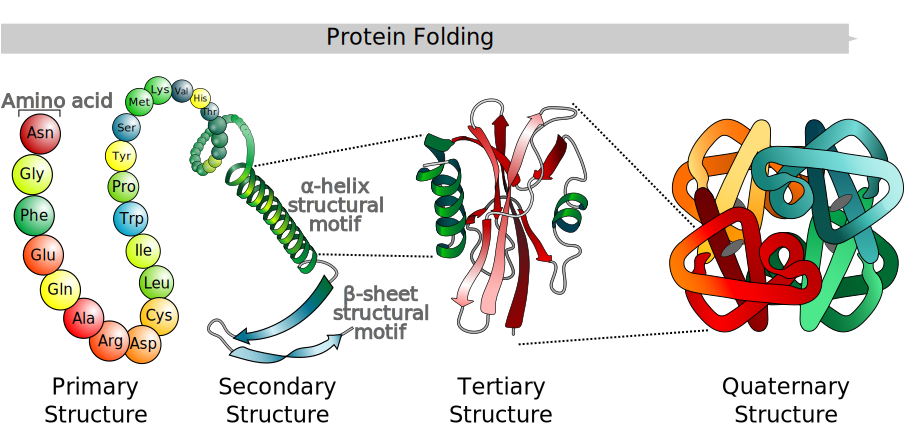
\includegraphics[width=0.95\textwidth]{villarreal_protein}
\caption[Protein structure]{\textbf{Protein structure.} Proteins are formed by building blocks termed amino acids. The chain of amino acids that forms a specific protein is the protein's primary structure. Protein secondary structures, such as $\alpha$-helixes or $\beta$-sheets, are formed through the natural folding of the amino acid chain given their physicochemical properties. The tertiary structure is composed of a number of secondary structures forming a stable protein unit. Finally, the quaternary structure represents the aggregation of multiple protein units to form fully functional protein. \emph{Source: Mariana R. Villarreal} (modified to fit thesis format and/or clarify key points).}
\label{fig:villarreal_protein}
\end{figure}

% Central dogma introduction
The process in which proteins are created based on the information encoded in the cell's DNA is called the ``central dogma of molecular biology''. Here, the key parts of this process, which aid in the understanding of this work, are presented. These key parts are: (1) the initiation, (2) the transcription and (3) the translation.

% Central dogma
During the initiation phase, a number of proteins called transcription factors (TFs) bind in the DNA and recruit another protein called RNA polymerase (Figure~\ref{fig:lodish_central_dogma}a). The DNA region in which these TFs and RNA polymerase bind to start transcription is called promoter. Then, in the transcription phase, the RNA polymerase scans the DNA and creates an RNA molecule, based on the information encoded in the DNA (Figure~\ref{fig:lodish_central_dogma}b). The part of the DNA which is transcribed by the RNA polymerase is called gene. Finally, in the translation phase, the newly-generated RNA migrates outside the cell's nucleus and a protein called ribosome scans the RNA and creates a new protein molecule based on the information encoded in the RNA (Figure~\ref{fig:lodish_central_dogma}c). The rate in which the transcription occurs for a particular gene is called the gene's expression.

% Transcription - strands and order
It is important to mention that, although only one of the DNA strands is read during the transcription process, both strands contain information necessary to produce RNA. Another important issue is the orientation of these two DNA strands. Each strand has two extremities: one corresponding to a hydroxyl group attached to the $3^\prime$ carbon atom of the sugar; and the other corresponding to the phosphate group attached to the $5^\prime$ carbon atom of the sugar. For this reason, processes involving the sliding of proteins in DNA have two orientations: forward ($5^\prime \rightarrow 3^\prime$) and reverse ($3^\prime \rightarrow 5^\prime$). The different strands in the DNA helix are attached to each other in opposite (anti-parallel) orientations. The transcription always occurs in the forward orientation.

% Figure - Central dogma of molecular biology
\begin{figure}[h!]
\centering
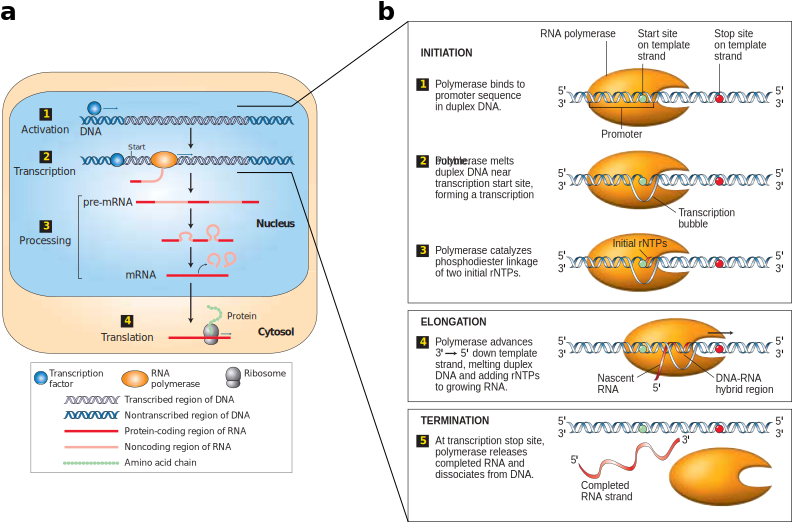
\includegraphics[width=0.99\textwidth]{lodish_30_central_dogma}
\caption[Central dogma of molecular biology]{\textbf{Central dogma of molecular biology.} Depiction of the main steps of the central dogma of molecular biology necessary to create a protein molecule from the information encoded within the DNA molecule. Here we show the steps: (\textbf{a}) initiation, (\textbf{b}) transcription and (\textbf{c}) translation. \emph{Source:~\cite{lodish2007}} (modified to fit thesis format and/or clarify key points).}
\label{fig:lodish_central_dogma}
\end{figure}

%%%%%%%%%%%%%%%%%%%%%%%%%%%%%%%%%%%%%%%%%%%%%%%%%%%%%%%%%%%%%%%%%%%%%
% Section: Eukaryotic Regulation
%%%%%%%%%%%%%%%%%%%%%%%%%%%%%%%%%%%%%%%%%%%%%%%%%%%%%%%%%%%%%%%%%%%%%
\subsection{Gene Regulation with Transcription Factors}
\label{sec:gene.regulation.transcription.factors}

% Introduction - Trascriptional regulation
The transcription initiation was previously described as the step in which the RNA polymerase binds to the promoter region in order to start the process of transcription. Nevertheless, there are many factors that contribute to the expression of particular genes in particular types/stages/conditions of a cell. We call ``gene regulation'' the wide range of mechanisms that are used by cells to increase or decrease the production of specific gene products. Gene regulation may happen in different stages of the central dogma. However, most part of the regulatory events happens at the transcription initiation level. A major role of the regulation at this level is played by proteins termed TFs, which use their physicochemical properties to direct the intensity level in which gene products are created. The TFs bind to DNA regions called TFBSs which are close (promoter region; approximately $< 1,000$ bp from the transcription start site) or far (distal regulatory regions; generally up to $1,000,000$ bp) from the gene. Different TFs may bind to different TFBSs to increase or decrease the expression of genes. Figure~\ref{fig:gusmao_gene_regulation} shows a graphical representation of a basic regulatory landscape of a gene. The number of regulatory elements vary between genes; however the construct of TF and their DNA binding sites are generally present.

% Figure - Regulatory elements
\begin{figure}[h!]
\centering
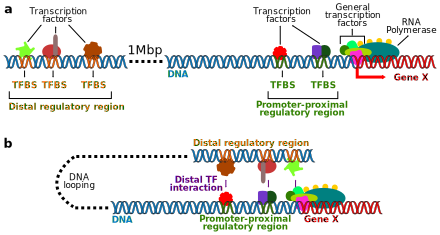
\includegraphics[width=0.95\textwidth]{gusmao_gene_regulation}
\caption[Basic regulatory landscape of a gene]{\textbf{Basic regulatory landscape of a gene.} (\textbf{a}) Schematic representation of a typical gene regulatory region with proximal and distal regulatory regions, composed of transcription factor binding sites (TFBSs), which are regions in the DNA being bound by proteins called transcription factors (TFs). The promoter typically spans less than $1$ Kbp and is composed of: (1) a core promoter -- where the transcriptional machinery is being bound and (2) promoter-proximal regulatory region -- where TFs bind to increase/decrease gene expression. The distal regulatory regions are located up to $1$ Mbp from the promoter. Among others, they are categorized as: (1) enhancers -- where TFs bind to increase gene expression and (2) silencers -- usually decreasing or completely silencing expression. (\textbf{b}) These distal elements may contact the core promoter or proximal promoter through a mechanism that involves looping out the intervening DNA. \emph{Based on~\cite{lodish2007}}.}
\label{fig:gusmao_gene_regulation}
\end{figure}

% Protein motifs
The TFs contain a specific part (formally called ``domains'') within their structure, termed active site, which enables them to bind to the DNA. There is a relatively short number of smaller structural variants (which compose the final protein structure) in comparison to the number of different protein types. Some of these structural variants, including the ones containing active sites, are repeated between different protein. These DNA-binding protein domains usually have affinities towards specific DNA sequences. These affinity sequences are termed ``DNA motifs''. Figure~\ref{fig:gusmao_binding_type} shows four DNA-binding protein domains and examples of proteins that contain such domains and their respective DNA binding affinity motifs.

% Figure - Different protein-DNA binding types
\begin{figure}[h!]
\centering
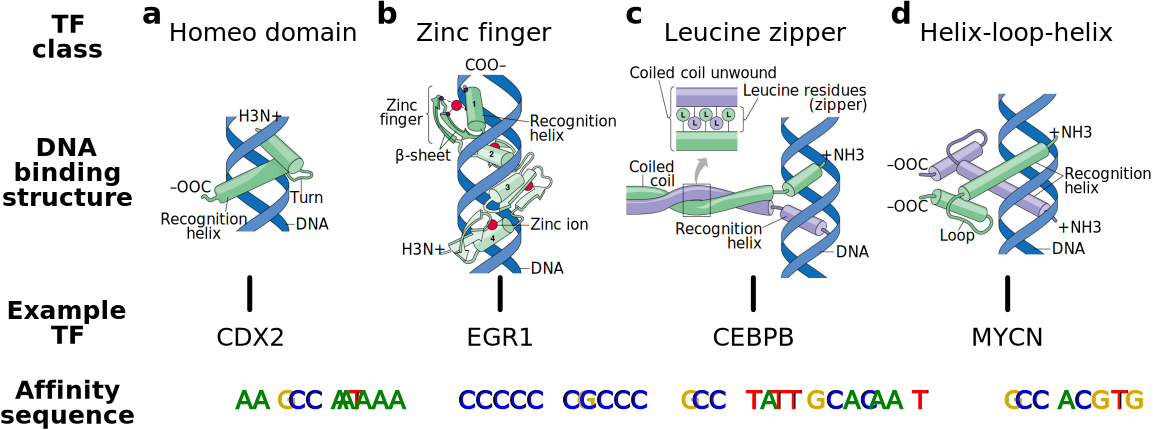
\includegraphics[width=0.99\textwidth]{gusmao_binding_type}
\caption[Different protein-DNA binding types]{\textbf{Different protein-DNA binding types.} We show graphical representations of different protein-DNA binding types (top) and examples of proteins with such binding domain type and their DNA sequence binding affinity information (bottom). We show four DNA-binding TF classes: (\textbf{a}) Homeo domain (also known as helix-turn-helix), (\textbf{b}) zinc finger, (\textbf{c}) leucine zipper and (\textbf{d}) helix-loop-helix. This motivates the idea that, although there are many DNA-binding proteins, they usually have a few DNA-binding domains. It is important to mention that, although we show only one affinity DNA sequence for each example, proteins have flexibility within some parts of their motif to bind different nucleotides. \emph{Source:~\cite{alberts2007}} (modified to fit thesis format and/or clarify key points).}
\label{fig:gusmao_binding_type}
\end{figure}

%%%%%%%%%%%%%%%%%%%%%%%%%%%%%%%%%%%%%%%%%%%%%%%%%%%%%%%%%%%%%%%%%%%%%
% Section: Chromatin
%%%%%%%%%%%%%%%%%%%%%%%%%%%%%%%%%%%%%%%%%%%%%%%%%%%%%%%%%%%%%%%%%%%%%
\subsection{Chromatin}
\label{sec:chromatin}

% Chromatin structure 1
The DNA is not isolated in the cell nucleus. Instead, it is found wrapped in proteic complexes, which are associated to the compaction of the DNA. The most important protein complex is formed by four pairs of histones named H2A, H2B, H3 and H4. The unit composed of the DNA wrapped in approximately $1.65$ turns (\approxy$147$ bp) around the histone complex is called nucleosome. From this lower level structure (nucleosome) the DNA structure is compacted in many levels. Such DNA$+$protein structure is termed chromatin. This compaction organization is depicted in Figure~\ref{fig:lodish_chromatin_structure}. Briefly, the chromatin can be found in a very condensed structure which does not allow transcription initiation (termed heterochromatin, or simply ``closed chromatin''); or in a decondensed form, allowing transcription initiation and gene expression (termed euchromatin, or simply ``open chromatin'').

% Figure - Chromatin conformation
\begin{figure}[h!]
\centering

\includegraphics[width=0.99\textwidth]{lodish_420_chromatin_structure}
\caption[Chromatin conformation]{\textbf{Chromatin conformation.} The nuclear DNA have many compaction levels. (\textbf{a}) The lowest chromatin level corresponds to the DNA double helix. (\textbf{b}) The DNA double helix loops around the histone complexes forming the nucleosomes. (\textbf{c}) With additional structural proteins, the nucleosomes are packed in a structure termed $30$-nm fiber. (\textbf{d}) The $30$-nm fiber is further compacted in many compaction levels with the aid of further structural proteins. (\textbf{e}) The higher degree of chromatin compaction is represented in the cell's metaphase. \emph{Source:~\cite{lodish2007}} (modified to fit thesis format and/or clarify key points).}
\label{fig:lodish_chromatin_structure}
\end{figure}

% Open / closed chromatin
Different parts of the genome are open or closed at different times, allowing a specific set of genes to be expressed under different cell conditions. This is one of the main mechanisms behind the fact that we observe such a high number of different cells, each of which expressing a different set of genes, given that they all share the same underlying genomic information encoded in the DNA. Figure~\ref{fig:lodish_open_closed_chromatin} shows a graphical example of two cells at different stages of commitment. Although the genomic region depicted is the same for these two cells, one present a closed chromatin structure, while the other present an open chromatin structure. The closed chromatin observed for the long-term hematopoietic stem cell (Figure~\ref{fig:lodish_open_closed_chromatin}a) does not allow the gene ATF3 to be transcribed, while the open chromatin structure present in the monocyte cell (Figure~\ref{fig:lodish_open_closed_chromatin}b) does allow the expression of ATF3 gene, since the TFs and transcription machinery are able to access that region and start the transcription process.

% Figure - Open vs closed chromatin
\begin{figure}[h!]
\centering
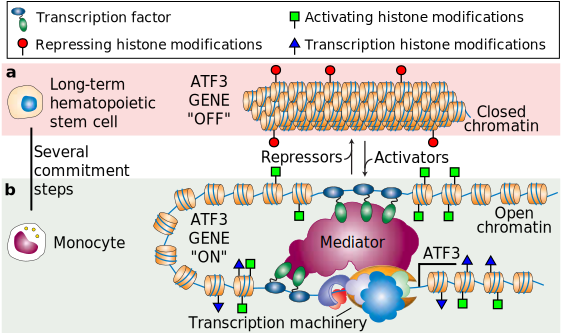
\includegraphics[width=0.83\textwidth]{lodish_461_open_closed_chromatin}
\caption[Open \emph{vs} closed chromatin]{\textbf{Open \emph{vs} closed chromatin.} Transription factor binding sites are cell-condition specific. This means that the same genomic locus might be accessible in a particular cell condition and not accessible in other condition. Such chromatin dynamics, which are modulated by genetic and epigenetic factors such as histone modifications, are responsible for the specialization of cells in performing the particular tasks required by the tissues they are located. This figure shows a graphical example of a locus (ATF3 gene) which is (\textbf{a}) closed in long-term hematopoietic stem cells (\textbf{b}) open in monocytes. Monocytes are a product of multiple specialization steps in hematopoietic stem cells. In this figure we show histone modifications which marks open/closed chromatin and proximal/distal regulatory regions. \emph{Source:~\cite{lodish2007}} (modified to fit thesis format and/or clarify key points).}
\label{fig:lodish_open_closed_chromatin}
\end{figure}

% Histone modifications
One of the main mechanisms associated to the chromatin switch between closed and open states is the post-translational histone modification. The histone proteins' N-terminal usually protrudes from the nucleosome and is termed histone tail. Histone tails can undergo post-translational chemical modifications at specific amino acids. Such modifications include the methylation (addition of a methyl group; labeled ``me'') and the acetylation (addition of an acetyl group; labeled ``ac''). These modifications have a specific nomenclature dictated by: histone type, amino acid type, amino acid position within the histone tail and modification type. For instance, ``H3K4me1'' refers to the monomethylation (me1) of the lysine (K) in the fourth position of the tail of histone H3. Some histone modifications, such as H3K4me3, make the DNA more accessible to the binding of TFs; while others, such as H3K27me3, make the DNA less accessible to the binding of TFs. Figure~\ref{fig:lall_histone_modifications} displays the different effects, on the chromatin structure, of modifications in lysines in the tail of histone H3.

% Figure - Main histone modifications on lysines of histone H3
\begin{figure}[h!]
\centering
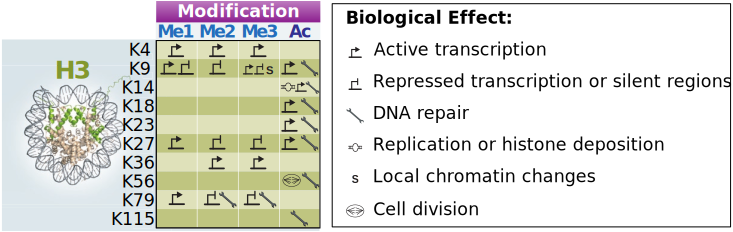
\includegraphics[width=0.95\textwidth]{lall_1111_histone_modifications}
\caption[Main histone modifications on lysines of histone H3]{\textbf{Main histone modifications on lysines of histone H3.} The tail of the histone H3 undergo post-translation modifications which are associated to chromatin remodeling. Different modifications at different locations of the H3's tail have contrasting effects such as transcription initiation or repression. \emph{Source:~\cite{lall2007}} (modified to fit thesis format and/or clarify key points).}
\label{fig:lall_histone_modifications}
\end{figure}


%%%%%%%%%%%%%%%%%%%%%%%%%%%%%%%%%%%%%%%%%%%%%%%%%%%%%%%%%%%%%%%%%%%%%
% Section: Next-Generation Sequencing Methods
%%%%%%%%%%%%%%%%%%%%%%%%%%%%%%%%%%%%%%%%%%%%%%%%%%%%%%%%%%%%%%%%%%%%%
\section{Next-Generation Sequencing Methods}
\label{sec:ngs.methods}

% Introduction
Recently, novel DNA sequencing platforms have enabled the sequencing of a very large number of DNA fragments (up to a few billions) on one single assay with a significant decrease in cost and complexity~\citep{hayden2014}. However, although these techniques are able to sequence a very large number of DNA fragments per single execution; these fragments are small (usually up to hundreds of bp). We call these novel sequencing platforms ``next-generation sequencing'' (NGS) techniques~\citep{shendure2008}. Since the development of the first NGS technologies~\citep{tucker2009}, they have been constantly improving. We refer to~\cite{rusk2010} for a full discussion on NGS technologies.

% Adapt old techniques
The emergence of NGS and its constant technological improvements have enabled the revisiting of traditional biological assays to investigate regulatory elements (described in Section~\ref{sec:gene.regulation.transcription.factors}) using the cell-specific chromatin dynamics context (described in Section~\ref{sec:chromatin}). On revisiting such methods, their protocols could be adapted in order to fit the NGS technologies, which enables them to be performed in a genome-wide manner. Such large-scale analysis has potential to reveal the high-dimensional relationships between regulatory elements. NGS-based assays have enabled multiple current research progress, which unraveled the regulatory mechanisms linked to conditions, such as cell differentiation or the onset of diseases, of multiple cells~\citep{encode2012,neph2012a,thurman2012}.

% This section
In this section we describe the following techniques: (1) Chromatin immunoprecipitation followed by NGS (ChIP-seq; Section~\ref{sec:chip.seq}) and (2) DNase I footprinting followed by NGS (DNase-seq; Section~\ref{sec:dnase.seq}). ChIP-seq combines chromatin immunoprecipitation with massively parallel DNA sequencing to identify the binding sites of DNA-associated proteins such as TFs or histones containing a particular modification. The DNase-seq method is used to identify regions of open chromatin, i.e. DNA regions accessible to the binding of TFs.

%%%%%%%%%%%%%%%%%%%%%%%%%%%%%%%%%%%%%%%%%%%%%%%%%%%%%%%%%%%%%%%%%%%%%
% Subsection: ChIP-seq
%%%%%%%%%%%%%%%%%%%%%%%%%%%%%%%%%%%%%%%%%%%%%%%%%%%%%%%%%%%%%%%%%%%%%
\subsection{ChIP-seq}
\label{sec:chip.seq}

% ChIP-seq introduction
The ChIP-seq technique consists on retrieving target DNA-bound proteins and further sequencing of the DNA fragments retrieved using NGS techniques~\citep{johnson2007}. These target proteins can be, for instance, TFs or histones with a particular post-translational modification. This allows the genome-wide identification of the genomic regions in which a target protein is bound within a single experimental execution. When applied to a target TF, the ChIP-seq experiment allows us to identify the TFBSs. When applied to histones with particular post-translational modification, the ChIP-seq experiment allows us to identify the genomic regions in which these modified histones occur, and therefore make inferences on that region's particular chromatin structure.

% ChIP-seq process
The ChIP-seq protocol starts by isolating the nuclei of cells and breaking them in order to access the genomic material (chromatin). The isolated genomic material is cross-linked in order to preserve all protein-DNA binding events. Next, the cross-linked chromatin is sheared into approximately $200$ bp DNA fragments. Afterwards, the chromatin lysate is treated with an antibody that targets a particular protein of interest. The solution is then immunoprecipitated. In this procedure, we retrieve only the sheared chromatin fragments that contains the protein of interest. The immunoprecipitated solution is separated and washed in order to keep only the DNA fragments. Then, these DNA fragments are sequenced using an NGS technique. It is important to mention that only the beginning of the retrieved DNA fragments are sequenced ($50$--$100$ bp) by NGS techniques. Such process is depicted in Figure~\ref{fig:gusmao_chipseq}a--c.

% ChIP-seq process - genomic signal
The sequenced DNA fragments (termed ``reads'') are mapped back into the reference genome using string alignment algorithms (Figure~\ref{fig:gusmao_chipseq}d), which are developed specially for mapping short DNA reads (length of $50$--$100$ bp) into a big reference genome (human genome length is \approxy$3.1$ billion bp). Such demanding computational problem is considered a solved problem and there are many available algorithms such as Bowtie~2~\citep{langmead2012} or the Burrows-Wheeler Aligner (BWA)~\citep{li2009b}. Given these aligned reads, we can generate a genomic signal by calculating the overlap between these reads at every genomic coordinate, i.e. every bp of the genome (Figure~\ref{fig:gusmao_chipseq}e--f). Nevertheless, since only the first $50$--$100$ bp of the fragments are sequenced, they need to be extended to reflect the real length of the immunoprecipitated fragments (approximately $200$ bp). This extension step reflects the fact that the protein is bound to virtually any location within the immunoprecipitated DNA fragment.

% ChIP-seq process - enrichment
Finally, we can identify the binding locations of the target protein by evaluating the genomic regions with more reads mapped than expected by chance (often referred to as ``enriched regions''). As shown in Figure~\ref{fig:gusmao_chipseq}f such regions with more ChIP-seq mapped reads than expected by chance can be seen as ``peaks'' in the signal generated by counting the number of mapped ChIP-seq reads in each genomic position (Figure~\ref{fig:gusmao_chipseq}g). The identification of significant peaks in ChIP-seq mapped reads is also a computational problem which was solved with the development of  genomic peak-calling algorithms such as the model-based analysis for ChIP-seq (MACS)~\citep{zhang2008}. Since the ChIP-seq signal has a low resolution, i.e. it is smoothed given the fact that we have to extend the aligned reads, the target protein is considered to be likely bound anywhere within the called peaks.

% Figure - Chromatin immunoprecipitation sequencing experimental technique (ChIP-seq)
\begin{figure}[h!]
\centering
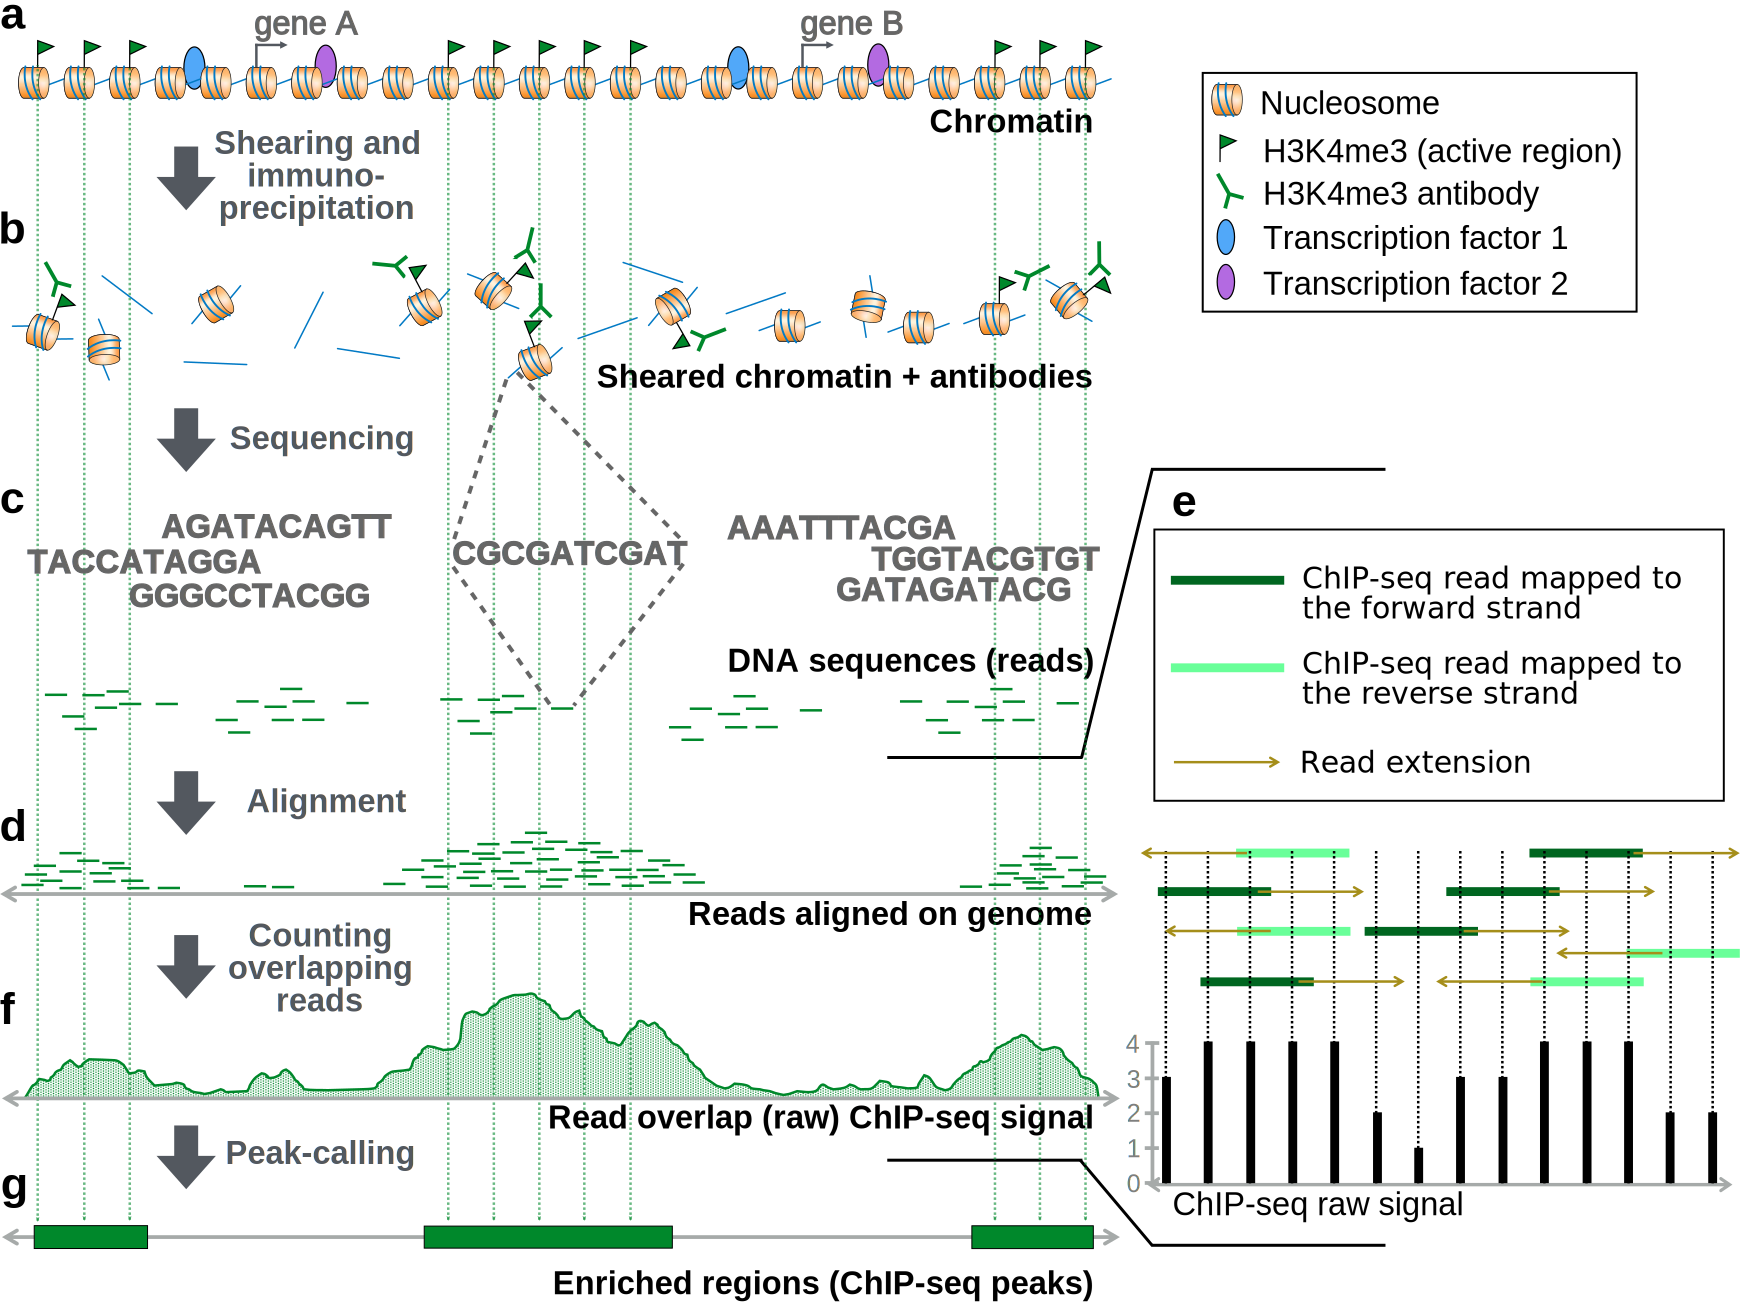
\includegraphics[width=0.99\textwidth]{gusmao_chipseq}
\caption[Chromatin immunoprecipitation sequencing experimental technique (ChIP-seq)]{\textbf{Chromatin immunoprecipitation sequencing experimental technique (ChIP-seq).} (\textbf{a}) The protocol starts by obtaining the chromatin from multiple cells. Such chromatin is cross-linked to preserve all protein-DNA interactions. (\textbf{b}) The cross-linked chromatin is sheared and treated with antibodies that target a particular protein of interest. The antibodies bind the target-protein and the chromatin fragments bound by these antibodies are recovered (immunoprecipitated). (\textbf{c}) The DNA fragments are sequenced using NGS-based techniques. Only the first $50$--$100$ bp of the \approxy$200$ bp fragments are sequenced. (\textbf{d}) The sequenced DNA fragments (reads) are mapped back into the reference genome using an alignment algorithm. (\textbf{e}) A genomic signal is generated by counting the overlap of the extended mapped reads. The reads are extended to match their original immunoprecipitated fragment length of \approxy$200$ bp. (\textbf{f}) The resulting genomic signal is enriched, i.e. present peaks, in the locations where the target protein is likely bound in the genome. (\textbf{g}) We can search for regions enriched with the ChIP-seq signal, which are the putative regions in which the target-protein is binding in the genome, using a peak-calling algorithm. \emph{Based on protocol description in~\cite{johnson2007}}.}
\label{fig:gusmao_chipseq}
\end{figure}

%%%%%%%%%%%%%%%%%%%%%%%%%%%%%%%%%%%%%%%%%%%%%%%%%%%%%%%%%%%%%%%%%%%%%
% Subsection: DNase-seq
%%%%%%%%%%%%%%%%%%%%%%%%%%%%%%%%%%%%%%%%%%%%%%%%%%%%%%%%%%%%%%%%%%%%%
\subsection{DNase-seq}
\label{sec:dnase.seq}

% DNase-seq intro
The DNase-seq technique consists in the observation of the DNA digestion by a certain cleavage agent able to break the DNA molecule~\citep{crawford2004,sabo2004a}. The cleavage agent used in this method is the enzyme deoxyribonuclease I (DNase I). The rationale of this method is that the DNase I enzyme can cleave the DNA in regions where it is accessible (i.e. open chromatin). Furthermore, within open chromatin regions, the DNase I enzyme cleaves the DNA only at protein-free regions, leaving ``footprint marks'' that can be traced back as DNA-bound (active) TFBSs.

% DNase-seq process - dnase I digestion & sequencing
The DNase-seq protocol starts by isolating the nuclei of cells and breaking them in order to access the genomic material (chromatin). The isolated genomic material is treated with optimal concentrations of DNase~I, which cleaves the chromatin at random accessible positions. These accessible positions are the chromatin regions in which the DNA is open (i.e. not fully wrapped around the histone complexes) and protein-free (i.e. not being bound by proteins such as TFs). Such cleaved DNA fragments are isolated and sequenced using the same algorithms as described for the ChIP-seq procedure (Section~\ref{sec:chip.seq}). Such process is depicted in Figure~\ref{fig:gusmao_dnaseseq}a--e.

% DNase-seq process - genomic signal
Then, a genomic signal is created by counting the number of overlapping reads at every genomic position. In the DNase-seq case, we only count the first base pair in the start ($5^{\prime}$ position) of the reads, since that is the position in which the DNase~I enzyme has cleaved the DNA and indicates an open chromatin region (Figure~\ref{fig:gusmao_dnaseseq}f--g). The resulting genomic signal represents a nucleotide-resolution map of the open chromatin positions within the whole genome.

% DNase-seq process - enriched regions and footprints
Finally, we can detect the genomic regions with more reads mapped than expected by chance, often referred to as ``DNase hypersensitivity sites'' (DHSs; Figure~\ref{fig:gusmao_dnaseseq}h). DHSs are detected by using algorithms specially designed for such purpose such as the F-seq~\citep{boyle2008b}. Each DHS is composed of several DNase-seq signal peaks. Note that the depletions within two of these nucleotide-resolution peaks are indicative of a region wherein the DNase~I enzyme could not access because there was a protein binding in that region. The DNase-seq signal depletion between two DNase-seq peaks is called a ``footprint'' (Figure~\ref{fig:gusmao_dnaseseq}h). The identification of footprints gives us a genome-wide map of putative active TFBSs.

% Figure - DNase I sequencing experimental technique (DNase-seq)
\begin{figure}[h!]
\centering
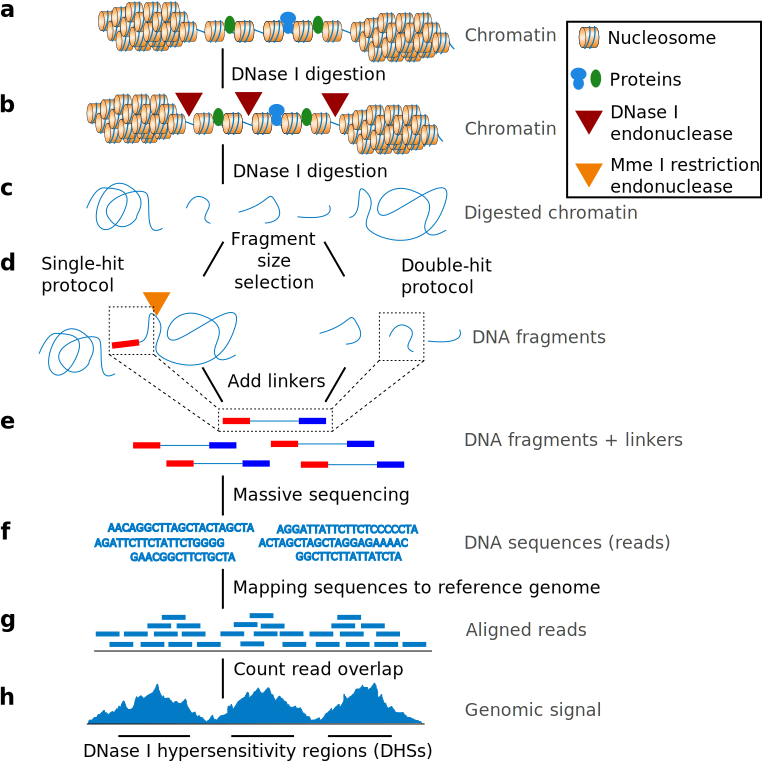
\includegraphics[width=0.83\textwidth]{gusmao_dnaseseq}
\caption[DNase I sequencing experimental technique (DNase-seq)]{\textbf{DNase I sequencing experimental technique (DNase-seq).} (\textbf{a}) The protocol starts by obtaining the chromatin from multiple cells. (\textbf{b}) The chromatin is treated with optimal levels of DNase I enzyme, which cleaves the chromatin in accessible sites. These accessible sites are the ones in which the chromatin is open and is not being bound by proteins (as TFs or histones). (\textbf{c}) After the DNase I digestion we have multiple fragments of sheared chromatin. The extremities of these fragments are isolated. (\textbf{d}) The isolated DNA fragments' extremities are sequenced using NGS-based techniques. (\textbf{e}) The aligned DNA sequences are mapped back into the reference genome. (\textbf{f}) A signal is generated by counting the overlap of the mapped DNA sequences. Since we are interested in the positions in which the DNase I enzyme has cleaved the DNA, only the first bp (i.e. $5^{\prime}$ bp) of the aligned read is count during the creation of the overlap signal. (\textbf{g}) The resulting read overlap signal exhibits peaks in the open chromatin (accessible to DNase I) regions. (\textbf{h}) Regions with high concentration of DNase-seq reads are termed DNase hypersensitivity sites (DHSs). Each of these regions are characterized by a number of depletions between peaks, which represent TF footprints. \emph{Based on protocol description in~\cite{crawford2004} and~\cite{sabo2004a}}.}
\label{fig:gusmao_dnaseseq}
\end{figure}

% Single-hit vs double-hit
There are two different protocols to perform the DNase-seq experiment, termed ``single-hit'' and ``double-hit''. There are a few experimental differences but the most important is the fragment size selection and isolation. While the single-hit DNase-seq protocol selects for larger cleaved fragments representing the extremities of the DHSs, the double-hit protocol selects for shorter cleaved fragments within the DHSs. Nevertheless, the resulting genomic signal and all post-read alignment steps are the same between these two approaches.

% DNase-seq vs ChIP-seq
It is important to point the differences between DNase-seq and ChIP-seq. In the DNase-seq method, we determine the binding of any protein in the region being analyzed, without knowing which protein is binding; however in ChIP-seq we only determine the binding of a particular target protein with a known antibody in the region of interest. Furthermore, while the DNase-seq can provide the precise protein binding location, the ChIP-seq tells us an approximated region for the binding of the target protein, since the protein binds virtually any \emph{locus} within the \approxy$200$ bp immunoprecipitated fragments. The selection of the technique to use depends mainly on the experimental design and should consider these important details.

%%%%%%%%%%%%%%%%%%%%%%%%%%%%%%%%%%%%%%%%%%%%%%%%%%%%%%%%%%%%%%%%%%%%%
% Section: Computational Prediction of Active TFBSs
%%%%%%%%%%%%%%%%%%%%%%%%%%%%%%%%%%%%%%%%%%%%%%%%%%%%%%%%%%%%%%%%%%%%%
\section{Computational Prediction of Active Transcription Factor Binding Sites}
\label{sec:computational.prediction.tfbs}

The identification of active TFBSs is a very important task, since they are the key players on most regulatory mechanisms. The detection of such regulatory elements have enabled significant advances in the understanding of many biological mechanisms such as cell differentiation~\citep{lin2015,tsankov2015} and the onset of diseases~\citep{schaub2012,vernot2012,charos2012}. In this thesis, we are going to address the computational prediction of active TFBSs.

The standard computational approach is the use of sequence-based methods, which search over the genome's DNA for sequences representing the DNA binding affinity sequence of TFs (Figure~\ref{fig:gusmao_binding_type})~\citep{stormo2000}. However, this approach is not able to predict active binding sites, i.e. binding sites that are being currently bound by TFs at a particular cell state (Section~\ref{sec:sequence.based.methods}). To introduce the cellular context, we can use the ChIP-seq for TFs (Section~\ref{sec:chipseq.tf}). However, success of ChIP-seq assays depends on the existence of a good antibody against the TFs of interest and on the availability of large numbers of cells. These two conditions are not always met in particular for primary cells. Furthermore, ChIP-seq is an expensive technique. Therefore, experiments involving ChIP-seq are restricted to the analysis of a small selection of TFs and cell types~\citep{kim2008,ouyang2009} or require the effort of large consortia~\citep{encode2012}. A solution to sequence-based and TF ChIP-seq-based methods' limitation is to explore the fact that an open chromatin structure is crucial and a prerequisite to the active binding of a TF on the DNA~\citep{arvey2012}. This solution is used by the computational chromatin-based methods (Section~\ref{sec:chromatin.based.method}).

%%%%%%%%%%%%%%%%%%%%%%%%%%%%%%%%%%%%%%%%%%%%%%%%%%%%%%%%%%%%%%%%%%%%%
% Subsection: Sequence-Based Methods \& Limitations
%%%%%%%%%%%%%%%%%%%%%%%%%%%%%%%%%%%%%%%%%%%%%%%%%%%%%%%%%%%%%%%%%%%%%
\subsection{Sequence-Based Methods \& Limitations}
\label{sec:sequence.based.methods}

% String matching
The standard computational approach to detect TFBSs is the use of sequence-based methods. These methods search the genome for the TF's DNA binding affinity motif~\citep{stormo2000}. Therefore, computational sequence-based methods to detect TFBSs can be viewed as string searching algorithms. The most common sequence-based approach is called motif matching. This algorithm scans the genome and scores every contiguous DNA sequence using a matrix representation of the TF's motif termed position frequency matrix (more details in Section~\ref{sec:motif.predicted.binding.sites}). The TFBSs predicted using computational sequence-based methods are called motif-predicted binding sites (MPBSs).

% Motif matching disadvantages
Computational sequence-based methods, such as the motif matching, have a low computational complexity, which makes their genome-wide application easy~\citep{mathelier2013}. However, while the genome is a large sequence of nucleotides (human genome length is \approxy$3.1$ billion bp), the TF's binding affinity sequences are small (usually between $5$--$20$ bp) and degenerate (only a fraction of the motif is highly conserved). Therefore, it is hard to fine-tune the sensitivity at the expense of the specificity~\citep{stormo2000}. Furthermore, this technique has a major disadvantage: it is unable to identify active binding sites, i.e. binding sites that are actually being bound by proteins at a specific cellular condition~\citep{boyle2011}. This happens because computational sequence-based methods rely solely on the DNA sequence affinity of proteins. However, the DNA sequence is the same between different cells for a particular organism; independent of cell type, cellular condition, life stage, stimuli response, and others. The key characteristic which allows different cells with the same genetic material to express a different set of proteins is the chromatin structure. Therefore, information regarding the chromatin structure is a prerequisite to identify active (cell type-specific) TFBSs~\citep{arvey2012,thurman2012}.

% Motif matching disadvantages
In practice, the fact that computational sequence-based approaches are unable to identify active binding sites is expressed as a very high number of false positive sequence-based predictions, representing the set of TFBSs not being accessed in a particular cellular condition. Figure~\ref{fig:gusmao_motif_match_problem} exemplifies this issue. We applied the motif matching tool ``find individual motif occurrences'' (FIMO)~\citep{grant2011} in a genomic region using $520$ TFs affinity representations with a conservative threshold to accept binding site hits. The result shows more than $3,000$ MPBSs on a $3,000$ bp region, which absolutely does not correspond to any possible biological regulatory model.

% Figure - Main problem of computational sequence-based methods
\begin{figure}[h!]
\centering
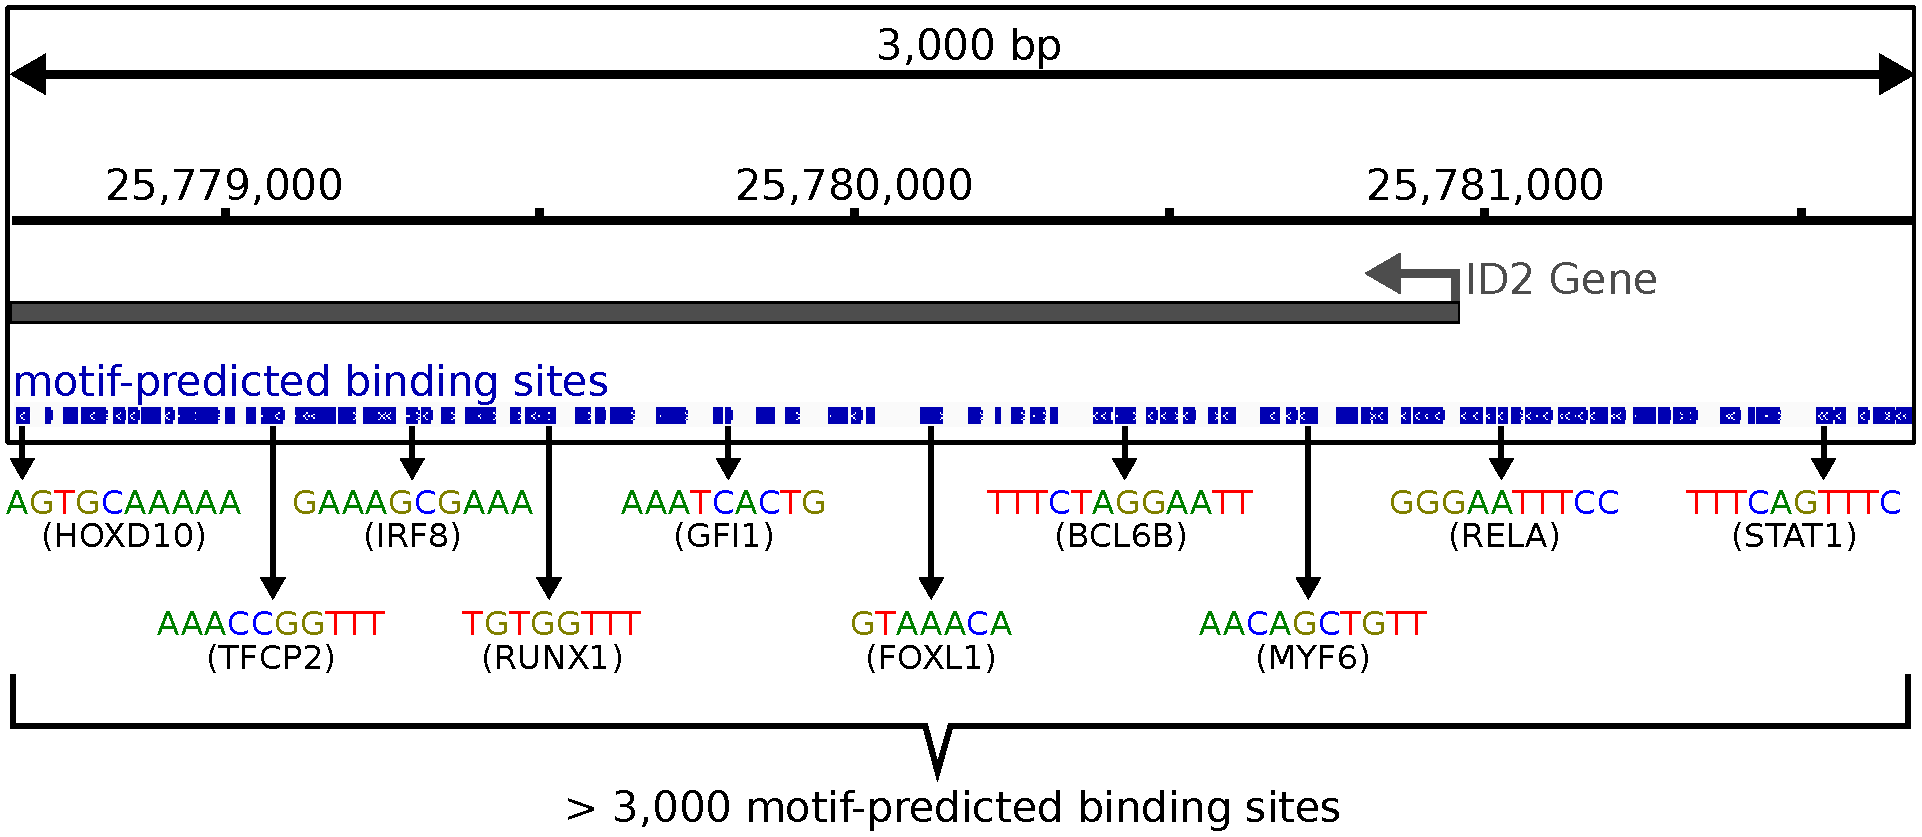
\includegraphics[width=0.99\textwidth]{gusmao_motif_match_problem}
\caption[Main problem of computational sequence-based methods]{\textbf{Main problem of computational sequence-based methods.} The motif matching tool FIMO~\citep{grant2011} was applied in a $3,000$ bp genomic region using $520$ TF DNA sequence binding affinity models and resulted in more than $3,000$ MPBSs. Such biologically impossible scenario exemplifies the fact that computational sequence-based approaches (such as motif matching) are, alone, unable to identify active binding sites.}
\label{fig:gusmao_motif_match_problem}
\end{figure}

%%%%%%%%%%%%%%%%%%%%%%%%%%%%%%%%%%%%%%%%%%%%%%%%%%%%%%%%%%%%%%%%%%%%%
% Subsection: ChIP-seq for Transcription Factors \& Limitations
%%%%%%%%%%%%%%%%%%%%%%%%%%%%%%%%%%%%%%%%%%%%%%%%%%%%%%%%%%%%%%%%%%%%%
\subsection{ChIP-seq for Transcription Factors}
\label{sec:chipseq.tf}

% Introduction
In order to make predictions of active TFBSs, we must use experimental data that give information on the chromatin dynamics and provide the required cell-specificity~\citep{arvey2012,thurman2012}. Such information is obtained with the biological assays discussed in Section~\ref{sec:ngs.methods}. 

% ChIP-seq
One way to obtain active TFBSs is to perform ChIP-seq on the target TFs of interest. Such assay provides all TFBSs for such target TFs with a very good accuracy and reasonable resolution.

% Disadvantages
However, using ChIP-seq to detect active TFBSs has a few limitations. First, the ChIP-seq relies on the quality of the antibody used on the immunoprecipitation step. There are many TFs in which the antibodies do not work properly or do not work at all. Second, if the experimental design relies on the identification of a small number of TFs ($<5$), then ChIP-seq for TFs might be a good experimental choice; however, if one is interested in a higher number of TFs, the number of TF ChIP-seq assays makes the study very expensive and time consuming~\citep{boyle2011,pique2011}.

%%%%%%%%%%%%%%%%%%%%%%%%%%%%%%%%%%%%%%%%%%%%%%%%%%%%%%%%%%%%%%%%%%%%%
% Subsection: Chromatin-Based Methods
%%%%%%%%%%%%%%%%%%%%%%%%%%%%%%%%%%%%%%%%%%%%%%%%%%%%%%%%%%%%%%%%%%%%%
\subsection{Chromatin-Based Methods}
\label{sec:chromatin.based.method}

% Using open chromatin markers
Given the limitations of ChIP-seq for TFs, a solution is to use experimental open chromatin data to narrow the search of active TFBSs. As previously discussed, histone modifications \emph{loci}, which are obtained using ChIP-seq, mark regions in which the chromatin is open, and therefore accessible to TFs~\citep{park2009}. Furthermore, the DNase-seq experimental assay provides open chromatin regions with a very high spatial specificity~\citep{boyle2008b}.

% Grammar of TFBSs
There is a distinctive pattern surrounding active TFBSs that is observed in genomic signals from DNase-seq and histone modification ChIP-seq. We refer to this pattern as the ``grammar of active TFBSs''~\citep{gusmao2012,gusmao2014}. This grammar, depicted in Figure~\ref{fig:gusmao_grammar_tfbs}, shows that TFBSs happen at depletions between two peaks of the DNase-seq signal (DNase footprints). These regions with multiple DNase-seq peaks, which comprise a DHS, occur within a depletion between two peaks of activating histone modifications (histone footprints)~\citep{boyle2011,gusmao2014}.

% Figure - Grammar of active TFBSs
\begin{figure}[h!]
\centering
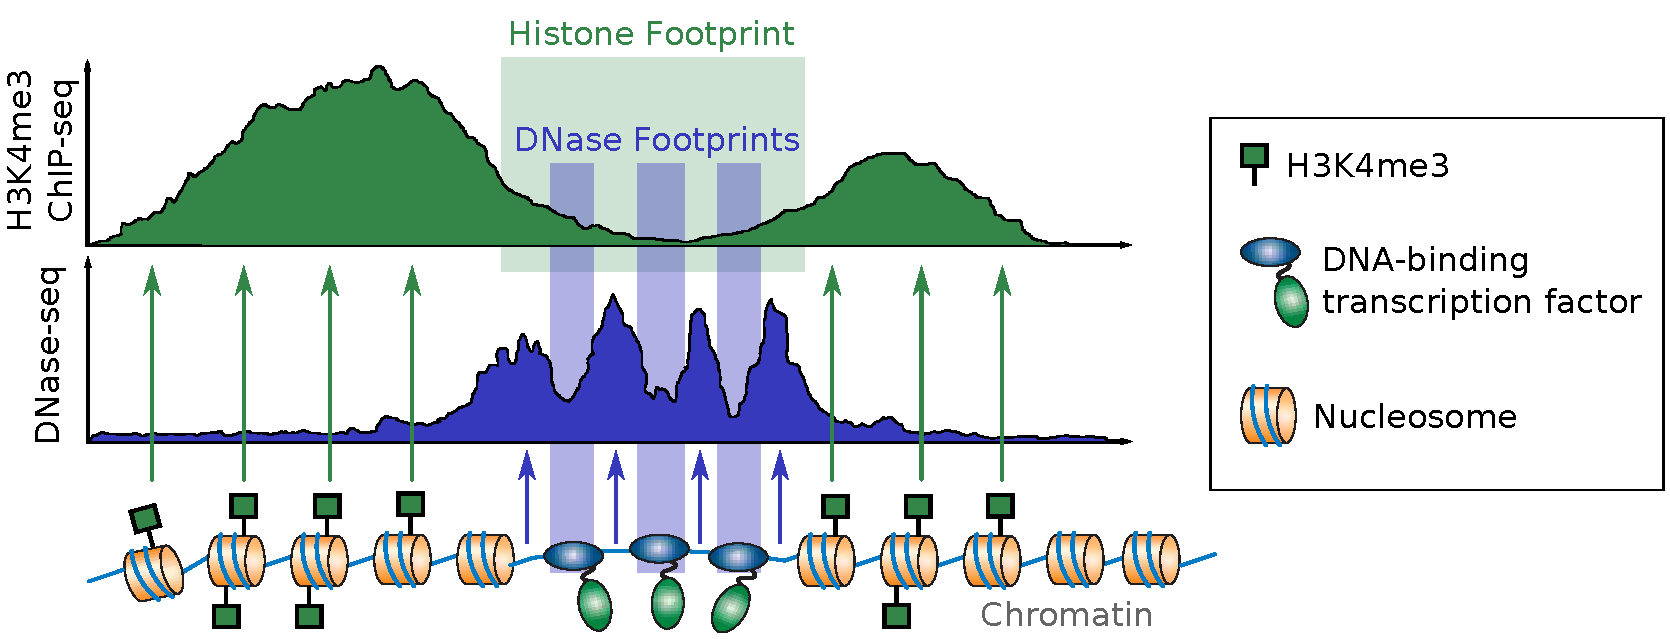
\includegraphics[width=0.99\textwidth]{gusmao_grammar_tfbs}
\caption[Grammar of active TFBSs]{\textbf{Grammar of active TFBSs.} In this figure we show examples of histone modification ChIP-seq and DNase-seq signals for a genomic region (top) and a graphical representation of the chromatin landscape within this region (bottom). We and others observed that there is a clear pattern regarding these signals and the TFBSs. TFBSs happen at depletions between two peaks of the DNase-seq signal (DNase footprints). Furthermore, these DNase-seq peaks, which determines an open chromatin region, happen at the depletion between two peaks of active histone modification marks (histone footprints).}
\label{fig:gusmao_grammar_tfbs}
\end{figure}

% Computational methods
Such patterns can be used in order to make better predictions of active binding sites, when compared to purely sequence-based methods~\citep{pique2011,cuellar2012}. Furthermore, a complete map of all putative active TFBSs, i.e. footprints, for a particular cell type can be obtained with a few assays (in the example of Figure~\ref{fig:gusmao_grammar_tfbs}, two assays: ChIP-seq for H3K4me3 and DNase-seq). However, the detection of footprints with DNase-seq and histone modification ChIP-seq require special computational frameworks. Such computational frameworks which processes open chromatin NGS-based data gained popularity over the last years and are used to address the problem of active TFBS prediction. Such chromatin-based computational methods that use open chromatin data to predict active binding sites are called ``computational footprinting methods'' and are the main subject of this thesis.

%%%%%%%%%%%%%%%%%%%%%%%%%%%%%%%%%%%%%%%%%%%%%%%%%%%%%%%%%%%%%%%%%%%%%
% Section: Computational Footprinting Methods
%%%%%%%%%%%%%%%%%%%%%%%%%%%%%%%%%%%%%%%%%%%%%%%%%%%%%%%%%%%%%%%%%%%%%
\section{Computational Footprinting Methods}
\label{sec:computational.footprinting.methods}

% This section
In this section we present the state-of-the-art computational methods, which use the grammar of active TFBSs to perform predictions of active TFBSs -- the computational footprinting methods (Section~\ref{sec:method.definition}). We define the different types of computational footprinting methods (Section~\ref{sec:types.computational.footprinting.methods}) and describe how they have been evaluated in the literature (Section~\ref{sec:evaluation.computational.footprinting.methods}). Next, we show the current challenges on the identification of active TFBSs using computational footprinting approaches (Section~\ref{sec:current.challenges}). Finally, we close this section with a comprehensive literature review on published computational footprinting methods (Section~\ref{sec:literature.review}).

%%%%%%%%%%%%%%%%%%%%%%%%%%%%%%%%%%%%%%%%%%%%%%%%%%%%%%%%%%%%%%%%%%%%%
% Subsection: Method Definition
%%%%%%%%%%%%%%%%%%%%%%%%%%%%%%%%%%%%%%%%%%%%%%%%%%%%%%%%%%%%%%%%%%%%%
\subsection{Method Definition}
\label{sec:method.definition}

% Introduction
In this thesis we focus on computational footprinting methods to address the problem of active TFBS prediction. We formalize the concept of computational footprinting method as follows:

\vspace{0.5cm}
\noindent
\textbf{Computational Footprinting Method:} \emph{A computational framework to analyze open chromatin (NGS-based) data and create a genome-wide map of active TFBSs.}
\vspace{0.45cm}

% Discussion of definition
The term ``computational framework'' refers to a set of methods and algorithms used to process the open chromatin data and perform the prediction of putative active TFBSs. Such computational framework has to be capable of executing within a reasonable amount of time with massive genome-wide data. Therefore, effort has to be done on applying efficient data structures and algorithms with minimal computational complexity. The output of computational footprinting methods consist of multiple genomic regions, each of which starts and ends at particular genomic coordinates, which represents the putative active binding sites. Furthermore, the predicted footprints should be as close as possible, in terms of genomic position and predicted region's width, to the real TFBSs. In other words, the method should have a high spatial specificity.

% The Footprint Score (FS) Method
\subsubsection{The Footprint Score (FS) Method}

% Footprint score 
The simplest computational footprinting approach, termed ``the footprint score (FS)''~\citep{neph2012a}, consists on sliding a window across the genome and evaluating the ratio between the number of reads (from a particular open chromatin experiment such as DNase-seq) inside the window and inside the flanking regions of the window (Figure~\ref{fig:gusmao_computational_footprinting}). More formally, let $\mathbf{x} = \langle x_1, \cdots, x_n \rangle$ be a genomic signal in which $x_i \in {\mathbb{N}}^{0}$ represents the number of DNase-seq mapped reads starting at the genomic position $i$ within a genome with total length $n$. The FS for a particular window represented as a genomic region $r_i = [u, v]$, which is an interval from the genomic coordinate $u$ to $v$ (including both), is calculated as
\begin{equation}
  \label{eq:fs1}
  \text{FS}_{r_i} = \left(\frac{{n}^{C}_{r_i}+1}{{n}^{R}_{r_i}+1} + \frac{{n}^{C}_{r_i}+1}{{n}^{L}_{r_i}+1}\right),
\end{equation}
where ${n}^{C}_{r_i}$, ${n}^{L}_{r_i}$ and ${n}^{R}_{r_i}$ are, respectively, the number of reads within, in the left and right flanking regions of the genomic region $r_i = [u, v]$. This is written as
\begin{align}
  \label{eq:fs2}
  {n}^{C}_{r_i} &= \sum_{j=u}^{v} {x}_{j}, &
  {n}^{R}_{r_i} &= \sum_{j=v}^{2v-u} {x}_{j}, &
  {n}^{L}_{r_i} &= \sum_{j=2u-v}^{u} {x}_{j}.
\end{align}

% FS
As depicted in Figure~\ref{fig:gusmao_computational_footprinting}, a negative $-\log \text{FS}_{r_i}$ indicates more reads (i.e. DNase I cleavage hits) in the core of the window $r_i$ than in its flanking regions. On the other hand, a positive $-\log \text{FS}_{r_i}$ indicates more reads in the window's flanking region in comparison with the core. As a consequence of the grammar of active TFBSs, we regard the regions with $-\log \text{FS}_{r_i} > t$, in which $t$ is a cutoff threshold, as the predicted footprints. This simple approach which relies on evaluating a score given a sliding window exemplifies the rationale behind computational footprinting methods. However, the problem with such window-based approach is that the length of the footprint is unknown and varies significantly between different proteins ($4$--$50$ bp)~\citep{neph2012a}. Furthermore, the length of the flanking regions, which in the FS method is the same as the length of the binding site, is also unknown and highly heterogeneous even with regard to the same TF~\citep{sung2014}.

% Figure - Simple example of computational footprinting
\begin{figure}[h!]
\centering
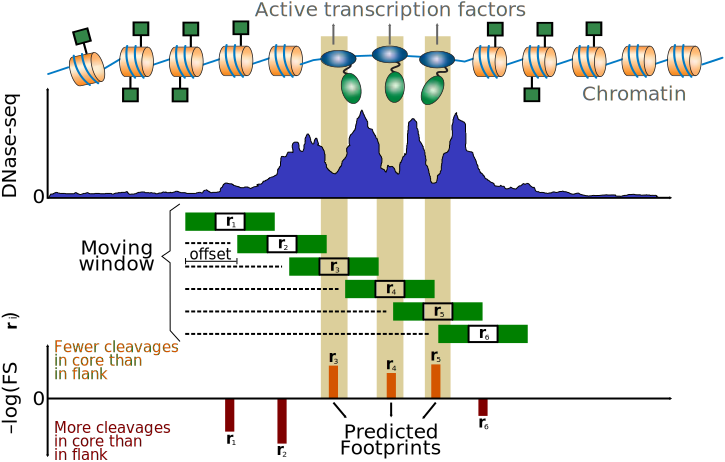
\includegraphics[width=0.85\textwidth]{gusmao_computational_footprinting}
\caption[Simple example of computational footprinting]{\textbf{Simple example of computational footprinting.} Depiction of a simple computational footprinting method which consists on sliding a window (denoted as $r_i$) composed of a core part (white box) and flanking regions (green box). The window, with a particular size, slides on the genome given a specific offset and corresponds to a predictive score. In the case of the FS shown in Equation~\ref{eq:fs1}, high positive $-\log \text{FS}_{r_i}$ values indicate footprints, which are putative active TFBS predictions.}
\label{fig:gusmao_computational_footprinting}
\end{figure}

%%%%%%%%%%%%%%%%%%%%%%%%%%%%%%%%%%%%%%%%%%%%%%%%%%%%%%%%%%%%%%%%%%%%%
% Section: Types of Computational Footprinting Methods
%%%%%%%%%%%%%%%%%%%%%%%%%%%%%%%%%%%%%%%%%%%%%%%%%%%%%%%%%%%%%%%%%%%%%
\subsection{Types of Computational Footprinting Methods}
\label{sec:types.computational.footprinting.methods}

% Segmentation methods
Computational footprinting methods are broadly categorized as: (1) segmentation methods and (2) site-centric methods (Figure~\ref{fig:gusmao_segmentation_vs_sitecentric}). The rationale behind segmentation methods is to scan the genome and use open chromatin data to segment the genome in open and closed chromatin regions. By measuring the different levels of histone modification ChIP-seq and/or DNase-seq signal intensity, the segmentation methods are able to identify patterns which correspond to the grammar of active TFBSs; consequently, detecting footprints in a genome-wide manner. This approach generates a map of putative active binding sites without specifying the TFs that are binding these regions. Although further processing is necessary in order to identify which particular TF bind to these putative binding sites; the advantage of such approach is that binding sites of unknown TFs can be detected. Figure~\ref{fig:gusmao_segmentation_vs_sitecentric}a shows an example of the segmentation computational footprinting approach. The example shown in this figure is similar to the FS shown in Figure~\ref{fig:gusmao_computational_footprinting}.

% Site-centric methods
On the other hand, site-centric methods (Figure~\ref{fig:gusmao_segmentation_vs_sitecentric}b) start with putative binding sites obtained by using, for instance, a sequence-based prediction method such as motif matching (Section~\ref{sec:sequence.based.methods}). Then, open chromatin experimental data around these \emph{a priori} predictions are gathered and classified, generally using unsupervised machine learning methods. This approach leads to footprints for target TFs. The advantage of such approach is that we already know which TFs are binding to the predicted footprints. However, the disadvantage is that it depends on the \emph{a priori} TF evidence (such as the DNA binding affinity motif), which is not always available. Consequently, site-centric techniques are only able to identify binding sites from well-known TFs.

% Computational complexity
Moreover, the computational complexity of the site-centric approach is larger than that of \linebreak segmentation-based methods. To assess the complexity in terms of the big-$\mathcal{O}$ notation, let $n$ be the length of the genome, $w$ be the length of a window in which footprints are being searched, $m$ be the number of TFs in which we are interested in analyzing and $h$ be the number of MPBSs found by applying a motif-matching algorithm. The segmentation approach requires the sliding of a window of length $w$ with offset of a fraction of $w$ (usually $\frac{1}{3}$ in the case of the FS method) in the genome of size $n$. Therefore, the segmentation approach is $\mathcal{O}(n+w)$. The site-centric approach first requires the application of the motif matching, which has complexity $\mathcal{O}(nw)$. Then, it performs a classification algorithm in each MPBS, which has complexity of at least $\mathcal{O}(wh)$. Finally, the site-centric approach performs this operation for each one of the $m$ TFs. Therefore, it has complexity of $\mathcal{O}(m(nw + wh)) = \mathcal{O}(m((n+h)w))$. In other words, the segmentation approach requires one execution per genome to provide footprint predictions for all putative TFBSs; the site-centric approach requires one genome-wide execution per TF. In practice, if one is interested on a genome-wide exploratory analysis (\approxy$500$--$1000$ TFs), the execution of site-centric methods requires a significant amount of computational time.

% Figure - Segmentation vs site-centric computational footprinting methods
\begin{figure}[h!]
\centering
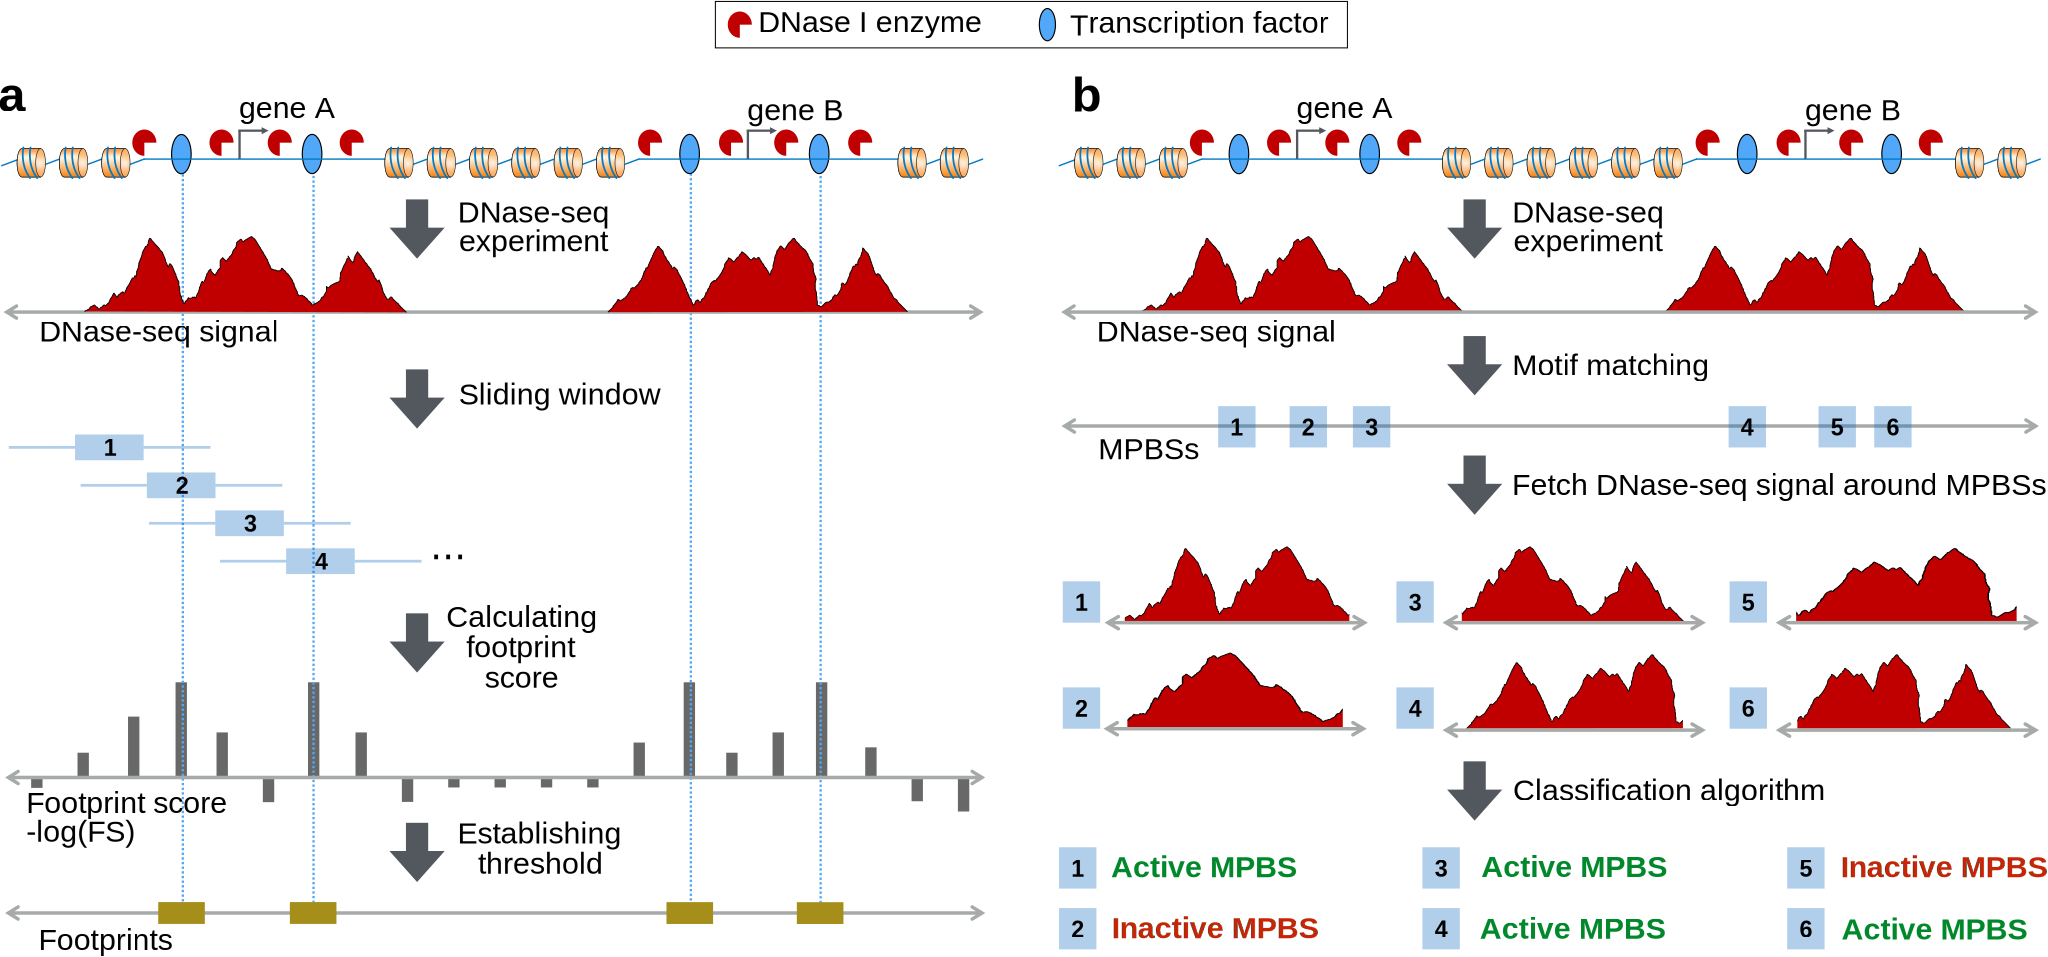
\includegraphics[width=0.99\textwidth]{gusmao_segmentation_vs_sitecentric}
\caption[Segmentation \emph{vs} site-centric computational footprinting methods]{\textbf{Segmentation \emph{vs} site-centric computational footprinting methods.} Example of each computational footprinting approach using DNase-seq data. Both approaches try to detect the grammar of active TFBSs. (\textbf{a}) The segmentation computational footprinting approach ``reads'' the DNase-seq signal as a time-series and searches for footprints based on the detection of patterns corresponding to the grammar of active TFBSs. In this case, the FS method is used as an example. The output of the segmentation approach corresponds to the genomic regions recognized as footprints. (\textbf{b}) The site-centric approach starts by detecting MPBSs using sequence-based algorithms such as motif matching. Then, the DNase-seq signal around all MPBSs is used to classify them as active/inactive binding sites. Such classification method distinguishes MPBSs that match the grammar of active TFBSs (active MPBSs) from the ones that do not (inactive MPBSs). In this case, the active MPBSs represent the footprint predictions.}
\label{fig:gusmao_segmentation_vs_sitecentric}
\end{figure}

%%%%%%%%%%%%%%%%%%%%%%%%%%%%%%%%%%%%%%%%%%%%%%%%%%%%%%%%%%%%%%%%%%%%%
% Section: Evaluation of Computational Footprinting Methods
%%%%%%%%%%%%%%%%%%%%%%%%%%%%%%%%%%%%%%%%%%%%%%%%%%%%%%%%%%%%%%%%%%%%%
\subsection{Evaluation of Computational Footprinting Methods}
\label{sec:evaluation.computational.footprinting.methods}

% Introduction
There is no well-defined gold standard for the evaluation of footprinting methods. All works so far have used ChIP-seq of TFs in conjunction with MPBSs as ground truth~\citep{pique2011,cuellar2012}. Such method provides a straightforward scenario for the evaluation of computational footprinting methods. The idea behind such an evaluation approach is that the TF ChIP-seq provides the cell-specificity and the MPBSs provides a countable structure which is used to calculate statistics. In the following we define such procedure.

% Procedure
In the so-called ``ChIP-seq evaluation approach'', MPBSs with ChIP-seq evidence (which can be, for instance, MPBSs close to TF ChIP-seq peak summits) are considered ``true'' TFBSs. On the other hand, MPBSs without ChIP-seq evidence are considered ``false'' TFBSs. Every TFBS prediction (i.e. footprint) that overlaps a true TFBS is considered a correct prediction (true positive -- TP) and every prediction that overlaps a false TFBS is considered an incorrect prediction (false positive -- FP). Therefore, true negatives (TN) and false negatives (FN) are, respectively, false and true TFBSs without overlapping predictions. This is depicted on Figure~\ref{fig:gusmao_chipseq_evaluation}a.

% ROC curves and AUC
The contingency table (TPs, FPs, TNs and FNs) enables the creation of receiver operating characteristic (ROC) curves, which describe the sensitivity increase as we decrease the specificity of the method (Figure~\ref{fig:gusmao_chipseq_evaluation}b). The area under the ROC curve (AUC) is a good metric to evaluate the overall performance of computational footprinting methods. Furthermore, the contingency table also enables the evaluation of the area under the precision-recall (PR) curve (AUPR; Figure~\ref{fig:gusmao_chipseq_evaluation}c). This metric is indicated for problems with imbalanced datasets (distinct number of positive and negative examples)~\citep{davis2006,fawcett2006}.

% Figure - Evaluation of computational footprinting
\begin{figure}[h!]
\centering
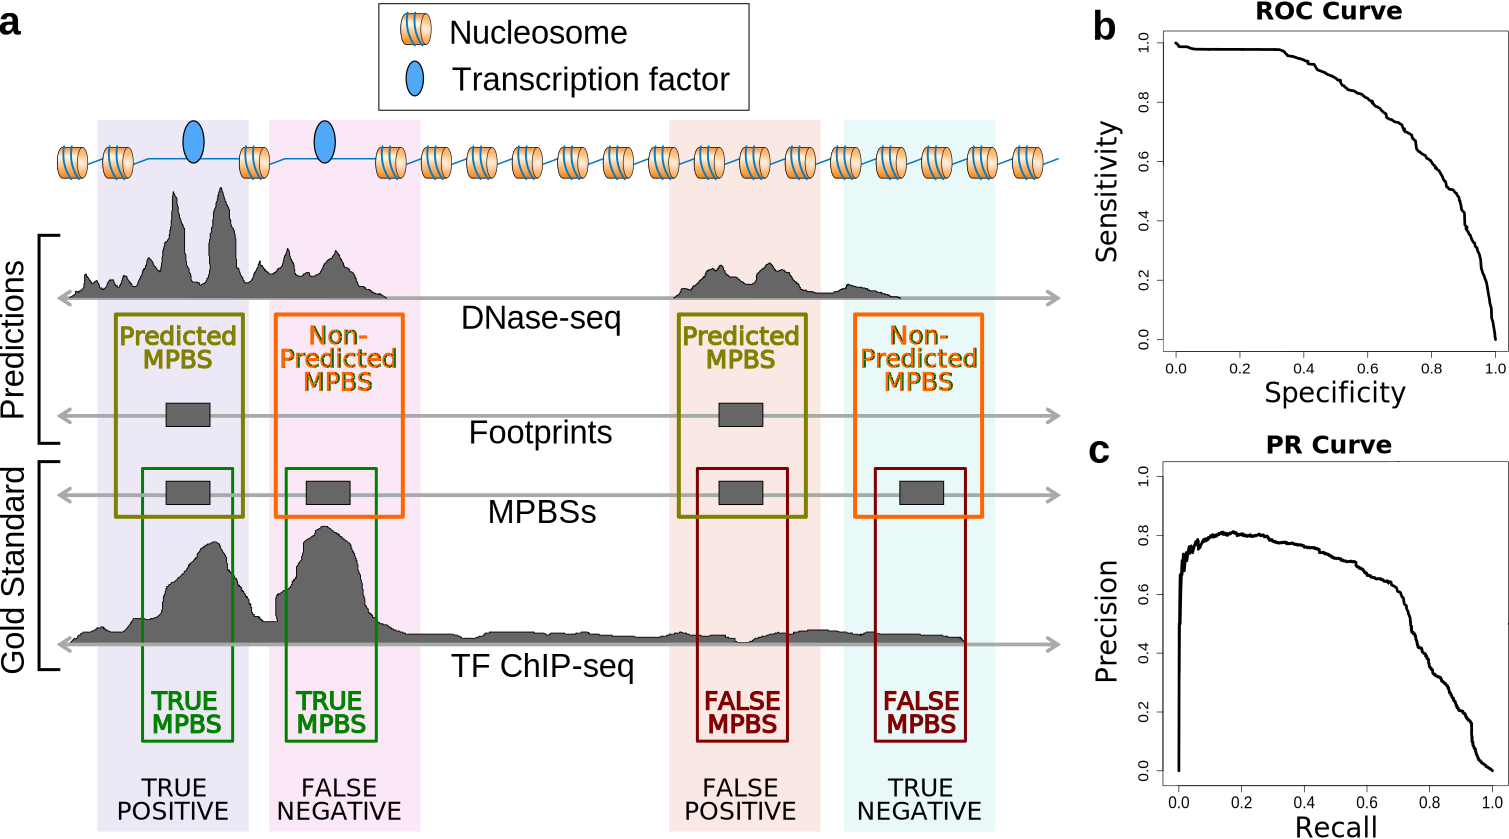
\includegraphics[width=0.99\textwidth]{gusmao_chipseq_evaluation}
\caption[Evaluation of computational footprinting]{\textbf{Evaluation of computational footprinting.} (\textbf{a}) In the ChIP-seq evaluation scheme, MPBSs for a particular TF are considered true if they are within a ChIP-seq enriched region for that particular TF. Otherwise, they are considered false MPBSs. By overlapping this information with footprint predictions from a particular computational footprinting method we are able to generate a contingency table with true positives, true negatives, false positives and false negatives. By ranking the MPBSs based on the overlapping footprint's quality, we are able to create: (\textbf{b}) receiver operating characteristic (ROC) curves and (\textbf{c}) precision-recall (PR) curves. These statistics can be used to rank computational footprinting methods and evaluate their overall performance on identifying each TF individually.}
\label{fig:gusmao_chipseq_evaluation}
\end{figure}

%%%%%%%%%%%%%%%%%%%%%%%%%%%%%%%%%%%%%%%%%%%%%%%%%%%%%%%%%%%%%%%%%%%%%
% Subsection: Current Challenges
%%%%%%%%%%%%%%%%%%%%%%%%%%%%%%%%%%%%%%%%%%%%%%%%%%%%%%%%%%%%%%%%%%%%%
\subsection{Current Challenges}
\label{sec:current.challenges}

% Introduction
There are a number of challenges in the development of computational footprinting methods for the identification of active TFBSs. Here we discuss current challenges which were not fully addressed by previous research studies. These challenges are the main motivations for the work presented in this thesis.

% Integration of Multiple Data Sources
\subsubsection{Integration of Multiple Data Sources}

% Integrative approaches
None of the computational footprinting methods published so far took advantage of the full-resolution spatial profile of all open chromatin NGS-based genomic signals. The current integrative approaches usually take only the full spatial signal for only one input data type. For instance, although a computational footprinting method called Centipede~\citep{pique2011} uses the full-resolution profile for the DNase-seq signal, it only uses averaged versions of the other signal types, such as histone modification ChIP-seq. Studies that considered some sort of integrative approach~\citep{pique2011,cuellar2012,sherwood2014,kahara2015} argue that the high degree of variation between different open chromatin NGS-based genomic signals makes their integration difficult and prone to overfitting. Furthermore, a number of computational footprinting methods used smoothed versions of the open chromatin data~\citep{cuellar2012,sherwood2014,kahara2015}. Therefore, the full spatial profiles from the integration of multiple sources of open chromatin data, such as DNase-seq and various histone modification ChIP-seq, has not been fully explored.

% Treatment of Intrinsic Experimental Bias on Open Chromatin Data
\subsubsection{Treatment of Intrinsic Experimental Bias on Open Chromatin Data}

% Signal treatment
It is known that open chromatin NGS-based genomic signals, such as DNase-seq and histone modification ChIP-seq, are noisy and intrinsically complex~\citep{meyer2014}. Most methods use smoothing techniques to handle such complexity~\citep{pique2011,cuellar2012,sherwood2014,kahara2015}. Although a few attempts have been made to use these signals in their maximum possible resolution~\citep{boyle2011,sung2014}, not much attention was given to data processing techniques such as signal normalization.

% Bias-correction
Furthermore, open chromatin NGS-based genomic signals are affected by multiple artifacts stemming from either the biological protocol or the computational pre-processing steps. These artifacts were summarized recently by~\cite{meyer2014}. \cite{he2014} showed that the DNase-seq sequence cleavage bias around TFBSs strongly affects the performance of the FS method, in a TF-specific manner. Such bias stems from the fact that the DNase I enzyme, used in the DNase-seq experimental technique, binds more often to certain DNA sequences than others. Since TFs also have a sequence binding preference (as depicted in Figure~\ref{fig:gusmao_binding_type}); the DNase-seq sequence cleavage bias might induce artificial footprints. This issue is observed, for the FS method, as a significant correlation between the amount of DNase-seq sequence cleavage bias surrounding each TF's binding sites and their computational footprinting prediction accuracies (Figure~\ref{fig:he_cleavage_bias}a).

% Bias profiles
\cite{he2014} also indicated several TFs, such as nuclear receptors, in which the DNase-seq footprint pattern resembles their DNase-seq sequence cleavage bias estimate. For instance, the average DNase-seq signal around binding sites of the transcription AR (androgen receptor) exhibits very similar patterns when a comparison is made between DNase-seq data from a cell type in which AR is known to be active (Figure~\ref{fig:he_cleavage_bias}b) and a cell type in which AR is known to be inactive (Figure~\ref{fig:he_cleavage_bias}c). 

% Figure - Impact of DNase-seq sequence cleavage bias on computational footprinting
\begin{figure}[h!]
\centering
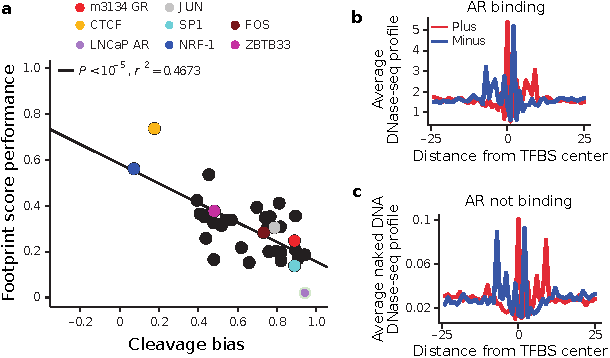
\includegraphics[width=0.90\textwidth]{he_5_cleavage_bias}
\caption[Impact of DNase-seq sequence cleavage bias on computational footprinting]{\textbf{Impact of DNase-seq sequence cleavage bias on computational footprinting.} (\textbf{a}) This graph shows the amount of DNase-seq sequence cleavage bias ($x$-axis) \emph{vs} the performance (AUC from the ChIP-seq evaluation approach) of the FS footprinting method. We clearly observe that there is a strong negative correlation between these two variables. (\textbf{b}) Average DNase-seq signal profile around ChIP-seq peaks of the AR TF in a cell type in which it is known that the AR TF is being expressed (i.e. AR is actively binding). (\textbf{c}) Average DNase-seq signal profile around the same regions as in (b); however in this case the DNase-seq is from a naked DNA experiment, where all proteins were removed from the DNA. In this case AR is not binding the DNA, but a footprint pattern can still be found. \emph{Source:~\cite{he2014}} (modified to fit thesis format and/or clarify key points).}
\label{fig:he_cleavage_bias}
\end{figure}

% Lack of Benchmark Data for Method Evaluation
\subsubsection{Lack of Benchmark Data for Method Evaluation}

% Lack of benchmark
Except for a few studies~\citep{sherwood2014, yardimci2014, kahara2015}, comparative analyses evaluating footprinting methods analyzed only a few ($<12$) TFs. Also, a maximum of only four competing methods were evaluated using the same experiment design of a particular published study. In addition, the experiment design for evaluation of computational footprinting methods vary between different publications. Despite the importance of method evaluation~\citep{rusk2015}, there is a clear lack of benchmark data, evaluation standards and studies performing a comprehensive analysis of computational footprinting methods.

% Evaluation - ChIP-seq bias
Furthermore, when we consider the few studies that performed comparative analyses so far, all of them have used the ChIP-seq evaluation scheme as described in Section~\ref{sec:evaluation.computational.footprinting.methods}. This evaluation requires TF ChIP-seq experiments to be carried out on the very same cells as the DNase-seq experiment and has a few caveats. First, TF ChIP-seq peaks are also observed in indirect binding events~\citep{yardimci2014}, i.e. a binding site might have ChIP-seq evidence of TF A when in fact it is actually binding TF B which is interacting with A by an indirect binding event, such as DNA looping. Second, they have a lower spatial resolution than DNase-seq. Consequently, false MPBSs might be regarded as true MPBSs by proximity to an active TFBS~\citep{cuellar2012,yardimci2014}. Therefore, it is important to devise a new evaluation strategy which does not rely on ChIP-seq data for independent evaluation of computational footprinting methods.

% Expression Evaluation
\cite{yardimci2014} proposed the use of gene expression data to evaluate footprint predictions using the following idea: the higher the expression of a particular TF in cell type A in comparison with cell type B, the higher the quality of the footprint predictions for that particular TF in cell type A (in comparison with B). Nevertheless, this evaluation strategy, which can be used to complement the ChIP-seq evaluation strategy, has not been systematically explored.

% Transcription Factor Binding Residence Time
\subsubsection{Transcription Factor Binding Residence Time}

% TF residence time 1
The open chromatin NGS-based techniques described in Section~\ref{sec:ngs.methods} also have constraints intrinsic to the regulatory mechanism of the cell. These experimental limitations were not fully explored in the light of computational footprinting method's performance. The main limitation regards the residence time of TFs binding on the DNA. \cite{sung2014} showed that short-lived TFs, i.e. TFs that have a low binding residence time, display a lower DNase-seq cleavage protection pattern, i.e. low number of DNase-seq mapped reads surrounding the footprint, when compared to a TF with higher binding residence time (Figure~\ref{fig:sung_residence_time}). Such fleeting TFs are harder to detect than other TFs with longer residence time since their protection pattern is less pronounced.

% TF residence time 2
Nevertheless, a systematic evaluation on the extent of the negative impact on footprint prediction accuracy given the TF binding residence time issue has not been made. It is very important to measure such impact to determine the feasibility of computational footprinting for certain TFs and cell types. Furthermore, a TF-wise quantification of such impact would assist in determining the overall quality of each TF's footprint predictions.

% Figure - TF residence time
\begin{figure}[h!]
\centering
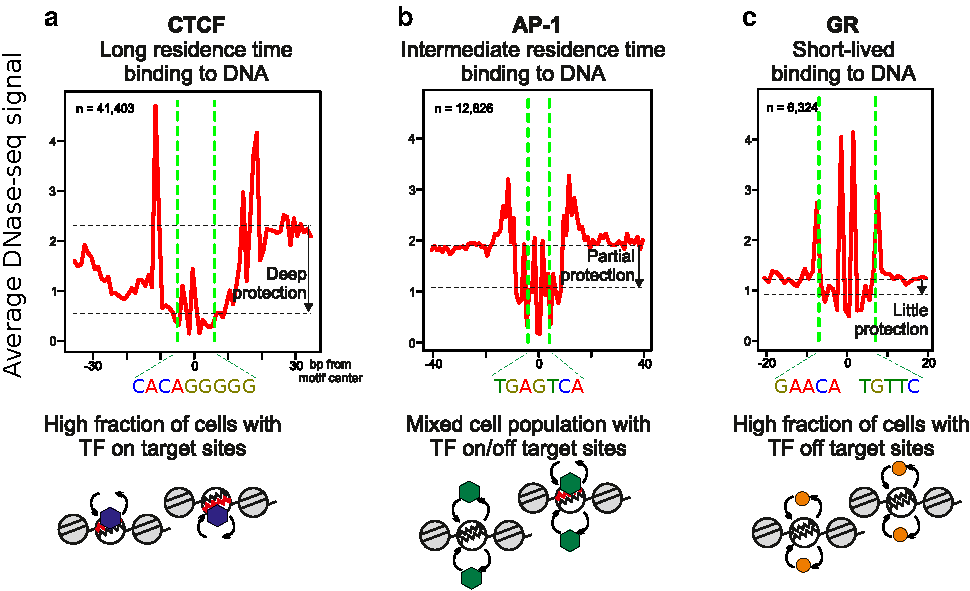
\includegraphics[width=0.95\textwidth]{sung_9_residence_time}
\caption[TF residence time]{\textbf{TF residence time.} This graphs depicts the average DNase-seq signal around TFBSs of TFs with: (\textbf{a}) long residence time -- CTCF; (\textbf{b}) intermediate residence time -- AP-1 (C-JUN) and (\textbf{c}) short residence time -- GR. \cite{sung2014} suggests that the DNase-seq signal width of the protection against the DNase I enzyme might be correlated with the residence time of TFs in the DNA. \emph{Source:~\cite{sung2014}} (modified to fit thesis format and/or clarify key points).}
\label{fig:sung_residence_time}
\end{figure}

%%%%%%%%%%%%%%%%%%%%%%%%%%%%%%%%%%%%%%%%%%%%%%%%%%%%%%%%%%%%%%%%%%%%%
% Section: Review on Computational Footprinting Methods
%%%%%%%%%%%%%%%%%%%%%%%%%%%%%%%%%%%%%%%%%%%%%%%%%%%%%%%%%%%%%%%%%%%%%
\subsection{Review on Computational Footprinting Methods}
\label{sec:literature.review}

% Introduction
A number of computational footprinting methods have been proposed. These methods use different combinations of open chromatin NGS-based experimental data sources, different algorithms and target different experiment designs. Here, we discuss the main published methods, providing a comprehensive literature review on computational footprinting methods.

%%%%%%%%%%%%%%%%%%%%%%%%%%%%%%%%%%%%%%%%%%%%%%%%%%%%%%%%%%%%%%%%%%%%%
% Section: Hesselberth et al.
%%%%%%%%%%%%%%%%%%%%%%%%%%%%%%%%%%%%%%%%%%%%%%%%%%%%%%%%%%%%%%%%%%%%%
\subsubsection{Hesselberth et al.}

% Hesselberth (hesselberth2009) - method (Hesselberth)
One of the first attempts to create a computational footprinting method for DNase-seq data was performed by~\cite{hesselberth2009}. In their study, they performed the DNase-seq experiment in the \emph{Saccharomyces cerevisiae} organism (yeast). They used a three-phase segmentation approach to detect footprints in the DNase-seq data. In the first phase, the authors consider every possible window that was contained within one of the specified target regions (DHSs) and compute a depletion score for each of these regions. The second phase consists of selecting high-scoring windows using a greedy algorithm, eliminating from consideration any window that overlapped a window with a higher score. Finally, in a third phase, the authors shuffle the input data independently within each target region and repeat the entire procedure, using the resulting scores to estimate quality scores. They introduced the FS (Equation~\ref{eq:fs1}) as a quality metric of footprints.

% Hesselberth (hesselberth2009) - results
Within this systematic identification of DNase-seq footprints,~\cite{hesselberth2009} analyzed many features regarding such footprint predictions. They identified many known sequence motifs in these footprints, observing that collectively, $35.2\%$ of the footprints with a false discovery rate of $0.05$ overlapped a conserved factor binding site inferred from ChIP-seq data. Furthermore, they observed that the patterns of DNase I protection surrounding different TFs had different average shapes, i.e. the DNase-seq average signal varies depending on the binding type of TFs. Finally, they created a very consistent genome-wide map of TFBSs for the \emph{Saccharomyces cerevisiae}, which led into insights on the chromatin architecture and gene expression of this organism.

%%%%%%%%%%%%%%%%%%%%%%%%%%%%%%%%%%%%%%%%%%%%%%%%%%%%%%%%%%%%%%%%%%%%%
% Section: Neph et al.
%%%%%%%%%%%%%%%%%%%%%%%%%%%%%%%%%%%%%%%%%%%%%%%%%%%%%%%%%%%%%%%%%%%%%
\subsubsection{Neph et al.}

% Neph (neph2012a)
\cite{neph2012a} used a simplified version of the segmentation-based method originally proposed in~\cite{hesselberth2009}. Their method consists on applying a sliding window to find genomic regions ($6$--$40$ bp) with low DNase-seq signal between regions ($3$--$10$ bp) with high DNase-seq signal (peak-dip-peak pattern). They performed their experiments on human DNase-seq data. They also use the FS to determine the most significant predictions. Their study amplified the analysis scale significantly, by detecting footprints for $41$ diverse human cells with data from the encyclopedia of DNA elements (ENCODE) repository~\citep{encode2012}. Such a large-scale study was able to provide multiple new insights on computational footprinting. First, they found that genetic variants affecting allelic chromatin states are concentrated in footprints, and that these elements are preferentially sheltered from DNA methylation. Second, they showed that the average TF-wise patterns of DNase I digestion is correlated to the crystallographic topography of protein-DNA interfaces, indicating that TF structure has been evolutionarily imprinted on the genome. Finally, they performed an extensive ``brute force'' \emph{de novo} motif finding algorithm and found $683$ unique DNA sequence affinity motif structures, of which $394$ ($58\%$) matched distinct experimentally-verified motif models present in Jaspar~\citep{mathelier2014}, Uniprobe~\citep{robasky2011} and Transfac~\citep{matys2006} motif repositories.

%%%%%%%%%%%%%%%%%%%%%%%%%%%%%%%%%%%%%%%%%%%%%%%%%%%%%%%%%%%%%%%%%%%%%
% Section: Boyle et al.
%%%%%%%%%%%%%%%%%%%%%%%%%%%%%%%%%%%%%%%%%%%%%%%%%%%%%%%%%%%%%%%%%%%%%
\subsubsection{Boyle et al.}

% Boyle (boyle2011)
\cite{boyle2011} designed a segmentation computational footprinting approach, which is based on using hidden Markov models (HMMs) to predict the DNase-seq pattern described in Figure~\ref{fig:gusmao_grammar_tfbs}. Briefly, their HMM uses a normalized DNase-seq signal to find regions with depleted DNase I digestion (footprints) between two peaks of intense DNase I cleavage. As the DNase-seq profiles required a nucleotide-resolution signal, which is usually noisy, the authors used a Savitzky-Golay smoothing filter to reduce noise and to estimate the slope of the DNase-seq signal~\citep{madden1978}. Their HMM had five states, with specific states to identify the decrease/increase of DHS signals around the peak-dip-peak region. They also provided numerous insights into computational footprinting. First, they described cell-specific footprint patterns, which correlate significantly with gene expression fold change between different cells. Second, they described a conservation phenomenon which was not observed in the conservation study performed by~\cite{hesselberth2009}. They find that for most TFs, there is a marked drop in conservation \approxy$10$ bp immediately flanking the footprint. Beyond this drop, conservation increases again before gradually decreasing to background levels, creating a ``shoulder'' in this signal. They also described in details the unique binding characteristics that the human insulator CTCF footprints displays. Finally, they used the STAMP~\citep{mahony2007} method to detect putative TFs in footprints, which simply searches for TFs on known DNA sequence affinity information. Therefore, a \emph{de novo} motif finding approach was not performed as in~\cite{neph2012a}.

%%%%%%%%%%%%%%%%%%%%%%%%%%%%%%%%%%%%%%%%%%%%%%%%%%%%%%%%%%%%%%%%%%%%%
% Section: Pique-Regi et al. (Centipede)
%%%%%%%%%%%%%%%%%%%%%%%%%%%%%%%%%%%%%%%%%%%%%%%%%%%%%%%%%%%%%%%%%%%%%
\subsubsection{Pique-Regi et al. (Centipede)}

% Pique-Regi (pique2011) (Centipede) 
One of the most common footprinting approaches was created by~\cite{pique2011}. Their strategy, termed Centipede, is a site-centric approach, which gathers experimental and genomic information around MPBSs. It then uses a Bayesian mixture model as an unsupervised classification tool to label each retrieved MPBS as either ``bound'' or ``unbound''. Their approach was the first to integrate multiple different experimental assays. The experimental data include DNase-seq and histone modification ChIP-seq. The DNase-seq data were used at its full spatial resolution (nucleotide-resolution), by obtaining raw DNase-seq signal surrounding a $200$ bp window around each MPBS. However, only the average histone modification ChIP-seq signal was used. The genomic data include the scores from the computational sequence-based approach used to create the MPBSs, sequence conservation and distance to the nearest gene. They evaluated their approach on six TFs with ChIP-seq data available, using the ChIP-seq evaluation approach. Their reported average AUC for the six tested TFs were as high as $98.11\%$. However, they did not observe a gain in accuracy when using a model with both DNase-seq and histone modification ChIP-seq (median AUC $= 96.52\%$).

%%%%%%%%%%%%%%%%%%%%%%%%%%%%%%%%%%%%%%%%%%%%%%%%%%%%%%%%%%%%%%%%%%%%%
% Section: Cuellar-Partida et al.
%%%%%%%%%%%%%%%%%%%%%%%%%%%%%%%%%%%%%%%%%%%%%%%%%%%%%%%%%%%%%%%%%%%%%
\subsubsection{Cuellar-Partida et al.}

% Cuellar (cuellar2012)
\cite{cuellar2012} proposed a site-centric method to include open chromatin NGS-based experimental data as priors for the motif matching procedure (Section~\ref{sec:sequence.based.methods}). Their method uses a probabilistic classification approach inspired in Bayes decision theory to compute better log-posterior odds scores than the ones observed by purely using the DNA sequence binding affinity model. Before the computation of prior probabilities the DNase-seq or histone modification ChIP-seq signals are smoothed as follows. To create smoothed DNase-seq signals they calculated the number of reads aligning to a window of $150$ bp, specified every $20$ bp. Histone modification smoothed signal input data was specified in a $25$ bp resolution. In every position, it was summed $ 1 $ if a mapped read fell within $0$--$200$ bp from the $25$ bp window and $ 0.25 $ if it occurred within $200$--$300$ bp. After the computation of prior probabilities with smoothed DNase-seq signal, they perform the motif match using the program FIMO~\citep{grant2011}. They performed the first comparative study on computational footprinting methods, where they compared their method with Centipede and with a much simpler approach termed ``tag count'' (TC). The TC approach, similar to the FS, consists on ranking the MPBSs using the number of DNase I cleavage hits within a window of length $l$ around the MPBSs. More formally, let the interval $r_i = [u, v]$ be the $i^{\text{th}}$ MPBS from a set $R$ of MPBSs and $\mathbf{x} = \langle x_1, ..., x_n\rangle$ be the DNase-seq genomic signal from a genome of size $n$. The TC for $r_i = [u, v]$ is calculated as 
\begin{equation}
  \label{eq:tc}
  \text{TC}_{r_i} = \sum_{j={\frac{u+v}{2}-\frac{l}{2}}}^{\frac{u+v}{2}+\frac{l}{2}-1} {x}_{j}.
\end{equation}

% Cuellar (cuellar2012)
Their results showed that, for their approach, the DNase-seq method dramatically improved the sequence-based prediction of TFBSs. Furthermore, they find that adding the histone modifications H3K4me3 or H3K27ac to their DNase-seq model improved the accuracy slightly. The comparison showed that Centipede outperformed their method using the gold standard proposed in~\cite{pique2011}. However, in this case, they found that using the simple TC approach would outperform both Centipede and their approach. They associate such results with the biases generated by such gold standard created on the basis of TF ChIP-seq data.

%%%%%%%%%%%%%%%%%%%%%%%%%%%%%%%%%%%%%%%%%%%%%%%%%%%%%%%%%%%%%%%%%%%%%
% Section: Piper et al. (Wellington)
%%%%%%%%%%%%%%%%%%%%%%%%%%%%%%%%%%%%%%%%%%%%%%%%%%%%%%%%%%%%%%%%%%%%%
\subsubsection{Piper et al. (Wellington)}

% Piper (piper2013) (Wellington)
\cite{piper2013} devised a segmentation approach based on a Binomial test. For a given candidate footprint, it tests the hypothesis that there are more reads in the flanking regions than within the footprint. Following an observation that DNase-seq cuts of the double-hit protocol are strand-specific, Wellington only considers reads mapped to the upstream flanking region of the footprints. They evaluate their method and competing methods in a ChIP-seq-based gold standard created with $214$ human TF ChIP-seq datasets. First, they showed that using such observed strand imbalance of reads increases the computational footprinting predictive power. Furthermore, their strategy outperformed the competing methods by~\cite{hesselberth2009},~\cite{neph2012a} and~\cite{pique2011}. Finally, this study performs a great contribution by creating a DNase-seq data processing package in the programming language Python termed pyDNase. Such package allows a user-friendly application of their methodology and also further DNase-seq data processing tools.

%%%%%%%%%%%%%%%%%%%%%%%%%%%%%%%%%%%%%%%%%%%%%%%%%%%%%%%%%%%%%%%%%%%%%
% Section: Sherwood et al. (PIQ)
%%%%%%%%%%%%%%%%%%%%%%%%%%%%%%%%%%%%%%%%%%%%%%%%%%%%%%%%%%%%%%%%%%%%%
\subsubsection{Sherwood et al. (PIQ)}

% Sherwood (sherwood2014) (PIQ)
\cite{sherwood2014} developed a computational footprinting framework termed protein interaction quantification (PIQ). PIQ is a site-centric method, which uses Gaussian process to model and smooth the footprint profiles around candidate MPBSs~\citep{sherwood2014}. Active footprints are estimated with an expectation propagation algorithm. Finally, PIQ indicates the set of motifs which footprint signals are distinguishable from noise to reduce the set of candidate TFs. They compared their method with competing methods in a very large benchmarking dataset containing $303$ TFs binding on K562 human cell type. Through the same evaluation procedure used in the aforementioned works~\citep{pique2011,cuellar2012,piper2013}, they measured a mean AUC of $0.93$ for PIQ against $0.87$ for Centipede~\citep{pique2011} and $0.65$ for Neph~\citep{neph2012a} approach.

% Sherwood further analyses
Nevertheless, this study contains many further analyses which provide insights into computational footprinting. They analyzed the differentiation of mouse embryonic stem cells into pancreatic and intestinal endoderm cells and were able to identify and experimentally validate eight pioneer TF families that perform changes in the chromatin dynamics. One of the most interesting findings is that these pioneer TFs change the chromatin directionally. Besides the identification of pioneer TFs, they also detected ``settler'' TFs, which binds the DNA after the chromatin structure changes performed by the pioneer TFs.

%%%%%%%%%%%%%%%%%%%%%%%%%%%%%%%%%%%%%%%%%%%%%%%%%%%%%%%%%%%%%%%%%%%%%
% Section: Yardimci et al. (FLR)
%%%%%%%%%%%%%%%%%%%%%%%%%%%%%%%%%%%%%%%%%%%%%%%%%%%%%%%%%%%%%%%%%%%%%
\subsubsection{Yard{\i}mc{\i} et al. (FLR)}

% Yardimci (yardimci2014) (FLR)
The issues on computational footprinting presented by~\cite{he2014} (Section~\ref{sec:current.challenges}) were analyzed in~\cite{yardimci2014}. In this study, they proposed a site-centric method (termed FLR) based on a mixture of multinomial models to classify MPBSs as active/inactive in an unsupervised manner. The method uses an expectation maximization algorithm to find a mixture of two multinomial distributions, representing active (footprints) and inactive (background) MPBSs. The background model is initialized with either DNase-seq sequence cleavage bias frequencies or estimated {\emph de novo}. After successful estimation, MPBSs are scored with the log odds ratio for the footprint \emph{vs} background model. The model takes DNase-seq cuts within a small window around the candidate profiles ($25$ bp up/downstream) as input. DNase-seq sequence cleavage bias is estimated for $6$-mers based on the DNA sequences extracted within the same regions in which the cuts were retrieved. They showed that their method significantly outperformed the simple TC approach. Furthermore, they also criticize the TF ChIP-seq evaluation method on the basis that it is not able to identify indirect binding events. For that reason, they performed a simple analysis based on gene expression and observed that the footprints retrieved by their approach are significantly enriched on cell types where the tested TFs are being expressed.

%%%%%%%%%%%%%%%%%%%%%%%%%%%%%%%%%%%%%%%%%%%%%%%%%%%%%%%%%%%%%%%%%%%%%
% Section: Sung et al. (DNase2TF)
%%%%%%%%%%%%%%%%%%%%%%%%%%%%%%%%%%%%%%%%%%%%%%%%%%%%%%%%%%%%%%%%%%%%%
\subsubsection{Sung et al. (DNase2TF)}

% Sung (sung2014) (DNase2TF)
\cite{sung2014} also performed a number of analysis that contributed to the discussion initiated in~\cite{he2014}. First, they developed a new segmentation computational footprinting approach with very simple premises, which is called DNase2TF. DNase2TF is based on the calculation of a binomial $z$-score based on the levels of DNase-seq depletion surrounding candidate footprints. At a second step, DNase2TF interactively merges close candidate footprints whenever they improve depletion scores. DNase2TF corrects for DNase-seq sequence cleavage bias using cleavage statistics for $2$ or $4$-mers. They reported that their method outperformed~\cite{hesselberth2009}, Centipede~\citep{pique2011} and Wellington~\citep{piper2013}. Furthermore, as~\cite{he2014}, they also raised the issue that some TF DNase-seq signatures resemble their cleavage bias. Moreover, they showed that one of the main problems with DNase-seq footprinting was related to the fact that some TFs have a very low residence time on DNA. Since they bind to the DNA in a short time period, the DNase-seq protocol is not able to produce a clear peak-dip-peak pattern.

%%%%%%%%%%%%%%%%%%%%%%%%%%%%%%%%%%%%%%%%%%%%%%%%%%%%%%%%%%%%%%%%%%%%%
% Section: Kahara et al. (BinDNase)
%%%%%%%%%%%%%%%%%%%%%%%%%%%%%%%%%%%%%%%%%%%%%%%%%%%%%%%%%%%%%%%%%%%%%
\subsubsection{K\"{a}h\"{a}r\"{a} et al. (BinDNase)}

% Kahara (kahara2015) (BinDNase)
\cite{kahara2015} developed a supervised site-centric method based on logistic regression to predict active/inactive MPBSs. The algorithm starts with nucleotide-resolution DNase-seq signal around the MPBSs ($100$ bps up/downstream) and selects discriminatory features using a backward greedy approach. As a supervised approach, the method requires positive and negative examples, which is obtained from TF ChIP-seq data. They showed that their approach does not present any significant gain in performance by modeling DNase-seq sequence cleavage bias. Furthermore, they present a discussion on the standardization of DNase-seq data pre-processing, showing that data on major repositories such as ENCODE are not always analyzed standardly. They state that their supervised approach outperforms unsupervised site-centric approaches such as Centipede~\citep{pique2011} and PIQ~\citep{sherwood2014}. However, since their approach is supervised (i.e. needs TF ChIP-seq data for model training), BinDNase is simply a sanity check for the TF ChIP-seq data. Therefore, it has little use in real-case scenarios and shares the same issues regarding the usage of TF ChIP-seq (Section~\ref{sec:chipseq.tf}).

%%%%%%%%%%%%%%%%%%%%%%%%%%%%%%%%%%%%%%%%%%%%%%%%%%%%%%%%%%%%%%%%%%%%%
% Section: Overview of Computational Footprinting Methods
%%%%%%%%%%%%%%%%%%%%%%%%%%%%%%%%%%%%%%%%%%%%%%%%%%%%%%%%%%%%%%%%%%%%%
\subsubsection{Overview of Computational Footprinting Methods}

% Overview of methods
In this section we made a comprehensive discussion on state-of-the-art computational footprinting methods. A summary of the main computational footprinting methods and their features is presented in Table~\ref{tab:overview_methods}. In this table we list the main characteristics of these computational footprinting methods:

\begin{itemize}
\item \textbf{Type.} The type of computational footprinting method: site-centric (SC) or segmentation (SEG).
\item \textbf{Algorithm.} The main algorithm that the method uses to perform footprint predictions.
\item \textbf{Bias Correction.} Whether the method performs DNase-seq sequence cleavage bias correction or does not perform such correction. Such correction estimates the sequence cleavage bias for all DNA sequences of length $k$ termed $k$-mers and use these bias estimates to correct footprint predictions.
\item \textbf{Resolution/Smoothing.} Whether the method applies a smoothing technique in the input open chromatin data or if it uses the full base-pair (bp) resolution data.
\item \textbf{Footprint Ranking.} The metric used to rank the footprint predictions. It is used as a quality metric to filter out lower-scored footprints.
\item \textbf{Availability.} The availability of software tool or source code. The methods obtain a `+' if they are public available (`--' otherwise).
\item \textbf{Usability.} Defines how complex it is to execute the method. The methods natively supporting standard genomic files and being executed with few commands ($\leq3$) have `+' (`--' otherwise).
\item \textbf{Others.} Other important additional information about the method.
\end{itemize}

% Table -  Overview of computational footprinting methods
\begin{footnotesize}
\begin{longtable}{p{1.4cm}p{0.6cm}p{1.7cm}p{1.3cm}p{1.6cm}p{1.6cm}p{0.8cm}p{0.8cm}p{2cm}}
\caption[Overview of computational footprinting methods]{\textbf{Overview of computational footprinting methods.} \emph{Source:~\cite{gusmao2016}} (modified to fit thesis format and/or clarify key points).} \\[-0.3cm]
  \hline
    Name & Type & Algorithm & Bias Correction & Resolution/ Smoothing & Footprint Ranking & Availa- bility & Usa- bility & Others\\
  \hline
    BinDNase & SC & Logistic Regression & No & bp / Sliding Window & Probability & + & -- & Require TF ChIP-seq for Training\\
    Boyle & SEG & HMM & No & bp & None & -- & -- & \\
    Centipede & SC & Bayesian Mix. Model & No & bp & Probability & + & -- & Integrates Histone and Sequence Data\\
    Cuellar & SC & Weighted Motif Match & no & Sliding Window & Sequence-based Score & + & -- & \\
    DNase2TF & SEG & Sliding Window & $4$-mer & bp & $p$-values & + & + & \\
    FLR & SC & Mixture Model & $6$-mer & bp & Log-Odds & + & -- & Bias Correction for Each TF\\
    Neph & SEG & Sliding Window & no & bp & FS & -- & -- & \\
    PIQ & SEG & GP/Expectation Propagation & No & bp / GP & Probability & + & + & Support Replicates, Time Series\\
    Wellington & SEG & Sliding Window & No & bp & $p$-value & + & + & \\
  \hline
\label{tab:overview_methods} \\
\end{longtable}
\end{footnotesize}

%%%%%%%%%%%%%%%%%%%%%%%%%%%%%%%%%%%%%%%%%%%%%%%%%%%%%%%%%%%%%%%%%%%%%
% Section: Discussion
%%%%%%%%%%%%%%%%%%%%%%%%%%%%%%%%%%%%%%%%%%%%%%%%%%%%%%%%%%%%%%%%%%%%%
\section{Discussion}
\label{sec:discussion.2}

% Summary
In this chapter we introduced the main concepts within the molecular biology field of gene regulation. Then, we defined the problem we are going to address in this thesis, which is to identify active TFBSs, i.e. DNA regions being bound by regulatory proteins at a particular cell state or condition. We have discussed that sequence-based computational approaches which takes advantage of the protein-DNA sequence binding affinity are not able to identify active sites, since the chromatin dynamics also needs to be considered. Nevertheless, we show that novel open chromatin assays such as DNase-seq and ChIP-seq capture such cell-specific chromatin dynamics. However, the magnitude and complexity of the data generated by these biological experimental assays call for robust computational frameworks. Finally, we discussed a particular type of computational framework for open chromatin data -- the computational footprinting methods -- which addresses the TFBS identification problem by processing such open chromatin data and searching for patterns that are indicative of active TFBSs. We performed a comprehensive literature review on the main computational footprinting methods and discussed the current challenges on this field.

% Plan for this thesis
In this thesis we investigate computational footprinting methods in detail. Among our goals are:
\begin{itemize}
\item The development of a computational footprinting method which takes advantage of the full (nucleotide-resolution) grammar of active TFBSs given by the DNase-seq and histone modification ChIP-seq data. Given the experimental flexibility of the footprints obtained using a segmentation-based approach, we are going to develop our method using the segmentation approach.
\item The investigation of techniques to process and normalize the DNase-seq and histone modification ChIP-seq signals. Furthermore, we will analyze the correction of the DNase-seq signal for DNase-seq sequence cleavage bias and other experimental artifacts, as these issues were correlated with a decrease in accuracy for other computational footprinting methods.
\item The comparison of multiple computational footprinting methods. We will investigate particularities associated to each method. Furthermore, we will analyze the correlation between the accuracy of computational footprinting methods and multiple biological genomic features. Moreover, we will also show the application our computational footprinting framework in real case scenarios.
\item The development of an alternative evaluation approach to that using TF ChIP-seq, to avoid interpreting the results only in the light of a single evaluation methodology. Furthermore, an attempt to create a benchmark dataset will be made, in order to standardize method comparison within this field. Such benchmark dataset and the comparative method analyses will be performed on a large compendium comprising many TFs, TF ChIP-seq data and gene expression data.
\item The investigation of the extent of the TF residence time's impact on footprint prediction performance. We plan to identify potential problematic TFs using only the input open chromatin data to assist in the biological interpretation of the computational footprinting methods' results.
\end{itemize}


